\documentclass[aspectratio=169]{beamer}

% ---------- Theme & Colors ----------
\usetheme{Madrid}
\usecolortheme{default}
\definecolor{tuwblue}{RGB}{0,86,145}
\definecolor{tuwdark}{RGB}{0,55,100}
\definecolor{tuworange}{RGB}{232,119,34}
\setbeamercolor{palette primary}{bg=tuwblue,fg=white}
\setbeamercolor{palette secondary}{bg=tuwdark,fg=white}
\setbeamercolor{palette tertiary}{bg=tuwblue,fg=white}
\setbeamercolor{palette quaternary}{bg=tuwdark,fg=white}
\setbeamercolor{structure}{fg=tuwblue}
\setbeamercolor{section in toc}{fg=tuwblue}
\setbeamercolor{alerted text}{fg=tuworange}
\setbeamertemplate{navigation symbols}{}

% ---------- Packages ----------
\usepackage{amsmath, amssymb}
\usepackage{booktabs}
\usepackage{graphicx}
\usepackage{xcolor}
\usepackage{tikz}
\usepackage{microtype}
\usepackage{listings}
\usepackage{array}
\usepackage[inkscapelatex=false]{svg}

% ---------- Code style ----------
\lstset{
  basicstyle=\ttfamily\footnotesize,
  keywordstyle=\color{tuwblue}\bfseries,
  commentstyle=\color{gray},
  breaklines=true,
  frame=single,
  rulecolor=\color{tuwblue!30}
}

% ---------- Footer ----------
\setbeamertemplate{footline}{%
  \leavevmode%
  \hbox{%
    \begin{beamercolorbox}[wd=.33\paperwidth,ht=2.25ex,dp=1ex,center]{author in head/foot}%
      \usebeamerfont{author in head/foot}Seifried \textperiodcentered{} Hagmann \textperiodcentered{} Rzecki
    \end{beamercolorbox}%
    \begin{beamercolorbox}[wd=.34\paperwidth,ht=2.25ex,dp=1ex,center]{title in head/foot}%
      \usebeamerfont{title in head/foot}BipedalWalker \& CartPole with DQN
    \end{beamercolorbox}%
    \begin{beamercolorbox}[wd=.33\paperwidth,ht=2.25ex,dp=1ex,right]{date in head/foot}%
      \usebeamerfont{date in head/foot}\insertframenumber{} / \inserttotalframenumber\hspace*{2ex}
    \end{beamercolorbox}}%
  \vskip0pt%
}

% ---------- New Section ----
\AtBeginSection[]{
    \begin{frame}
        \centering
        \vfill
        \Huge\insertsection
        \vfill
    \end{frame}
}

% ---------- Title ----------
\title[BipedalWalker with DQN]{%
  Deep Reinforcement Learning:\\
  \large Bipedal Walker \& Cart Pole with DQN
}
\subtitle{Introduction to Deep Learning --- Project 21}
\author[Seifried \textperiodcentered{} Hagmann \textperiodcentered{} Rzecki]{%
  Lea Seifried \and Michael Hagmann \and Dominik Rzecki
}
\institute{Technical University of Vienna}
\date{March 24, 2026}

% ==========================================================
\begin{document}
% ==========================================================

\begin{frame}
  \titlepage
\end{frame}

% ----------------------------------------------------------
\begin{frame}{Outline}
  \tableofcontents
\end{frame}

% ==========================================================
\section{Introduction and Overview}
% ==========================================================

\begin{frame}{Problems and Agents}
  Train agent, such that it solves a specific Problem ($\Leftrightarrow$ performs Task).
  \vspace{0.7em}
  \begin{columns}[c]
    \column{0.55\textwidth}
      \textbf{Agents Problem:} Perform that task correctly.
      \vspace{1.5em}

      \textbf{Engineers Problem:} Train such agent with least amount of effort. 
      \vspace{1.5em}

      $\Rightarrow$ \textbf{RL}

    \column{0.42\textwidth}
      \centering
      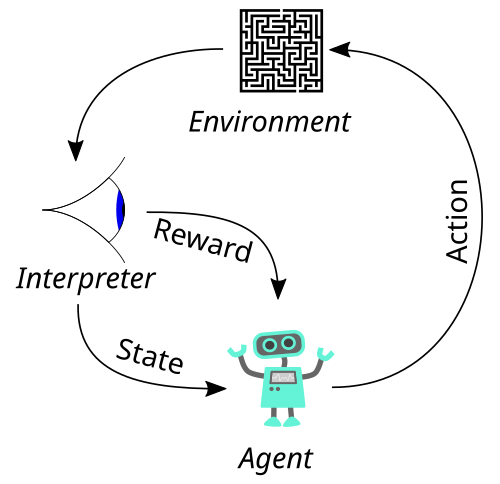
\includegraphics[width=\linewidth]{img/RLagent.png}
  \end{columns}
\end{frame}

\begin{frame}{Our Main Problem: Bipedal Walker from Gymnasium}
  Make stickman walk.
  \vspace{0.7em}
  \begin{columns}[c]
    \column{0.35\textwidth}
      \centering
      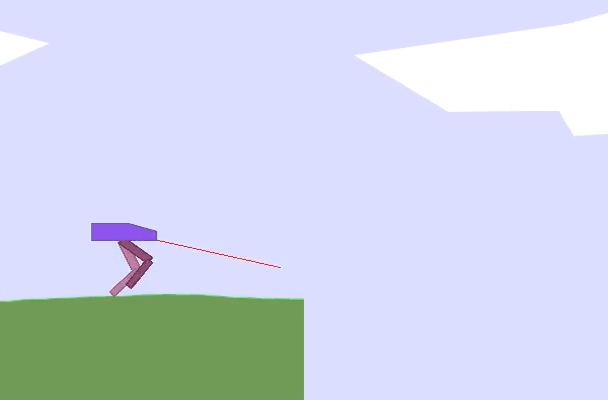
\includegraphics[width=\linewidth]{img/BipedalThumbnail.png}
    \column{0.6\textwidth}
      \textbf{Environment:}
      \begin{itemize}
        \item Flat slightly uneven slab, Newtonian Physics
      \end{itemize}
      \textbf{Agent:}
      \begin{itemize}
        \item lives in 2D
        \item 4 controllable joints (speed)
      \end{itemize}
      $\Rightarrow$ 6 total d.o.f., 4 controllable \\

      \vspace{0.7em}
      \textbf{Observation:}
      Hull angle, angular velocity, linear velocities ($x$, $y$),
      Joint angles \& angular velocities,
      Binary ground-contact info
      10 LIDAR range measurements \\
      \textbf{$\Rightarrow$ 24-dimensions} \\
  \end{columns}
\end{frame}

\begin{frame}{Rewards, Penalties \& No-Gos}
  Gymnasium provides interpreter. 
  \vspace{0.7em}
  \begin{columns}[c]
    \column{0.5\textwidth}
      \textbf{Reward components:}
      \begin{itemize}
        \item[\color{tuwblue}+] Positive reward for \alert{forward displacement}
        \item[\color{red}$-$] Large penalty ($-100$) for \alert{falling}
        \item[\color{orange}$-$] Small penalties for \alert{motor usage} (energy cost)
      \end{itemize}
    \column{0.47\textwidth}
      \begin{block}{Episode terminates when\ldots}
        \begin{enumerate}
          \item Torso contacts the ground (fall)
          \item End of terrain is reached
          \item Time limit exceeded
        \end{enumerate}
      \end{block}
      \vspace{0.5em}
      \begin{block}{Objective}
        Maximize cumulative discounted reward — keep walking, don't fall.
      \end{block}
      \vspace{1em}
      (We created Wrapper with reward shaping, more on that later.)
  \end{columns}
\end{frame}

\begin{frame}{Our Approach: Deep Q-Networks}
  \begin{columns}[c]
      \column{0.45\textwidth}
      {
        \textbf{(tabular)-RL:}
        \begin{itemize}
          \item Optimize sequential decision-making, under uncertainity through interaction and feedback.
          \item memorization, no compression (inf. obs. space $\Rightarrow$ inf. LUT)
        \end{itemize}
        \textbf{DNN/MLP:}
        \begin{itemize}
          \item Universal function approximation
          \item {Can compress / generalize. \\
            $\Rightarrow$ continous observation space
          }
        \end{itemize}
      }

    \column{0.1\textwidth}
      \centering
      {
        \Huge $\Rightarrow$
      }

    \column{0.45\textwidth}
      {
        \textbf{DQN:} (RL + DNN)
        \begin{itemize}
          \item Replace table with DNN to approximate $Q^*$
          \item Use Q-Function. (no model / policy derivation needed)
          \item[$\Rightarrow$]  continous observation space, generalization
          \item[$\Rightarrow$]  still discrete action space :(
          \item[$\Rightarrow$]  challanges: sample efficiency, stability
        \end{itemize}
      }
  \end{columns}
\end{frame}

% ==========================================================
\section{Theoretical Background}
% ==========================================================

\begin{frame}{Reinforcement Learning: Core Concepts}
  \begin{columns}[c]
    \column{0.52\textwidth}
      \textbf{Markov Decision Process $(S,A,P,R,\gamma)$: }
      \[s_1,a_1,r_1,\;s_2,a_2,r_2,\;\ldots\]

      \begin{itemize}
        \item \textbf{$s_i \in S$} State
        \item \textbf{$a_i \in A$} Action
        \item \textbf{$r_i \sim R(s_i, a_i)$} Reward
        \item $P(s'|s,a)$ Transition Probabilities
      \end{itemize}

      \textbf{Discounted Return:}
      \[G_t = \sum_{k=0}^{\infty}\gamma^k r_{t+k+1}, \quad \gamma \in [0,1)\]

    \column{0.45\textwidth}
      \textbf{Policy $\pi(a|s)$}: \textbf{Learned} mapping from states to a distribution over actions.
      \vspace{1.0em}

      \textbf{Objective:} Find a $\pi(a|s)$, such that $\mathbb{E}[G_t]$ is maximized.  
      \vspace{1.0em}
      
      DQN is \alert{model-free} — no access to model dynamics $P(s'|s,a)$. 
  \end{columns}
\end{frame}

\begin{frame}[t]{Q-Learning: Action-Value Function}

\textbf{Goal:} Estimate the return \(G_t\) during a trajectory, i.e., learn the ``goodness'' of a state-action pair \((s_t, a_t)\).

  \vspace{1em}
  \textbf{Action-value function (policy-dependent):}
  \[
  Q^\pi(s,a) = \mathbb{E}_\pi \left[ G_t \mid s_t = s, a_t = a \right]
  \]

  \vspace{1em}
  \textbf{Optimal action-value function:}
  \[
  Q^*(s,a) = \max_\pi Q^\pi(s,a)
  \]
  \vspace{0.5em}

\end{frame}

\begin{frame}{DQN Learning: Bellman Target \& Loss}

  \textbf{Bellman optimality equation:}
  \[
  Q^*(s,a) =
  \mathbb{E}\left[
  r_{t+1} + \gamma \max_{a'} Q^*(s_{t+1}, a')
  \right]
  \]

  \vspace{0.8em}

  \textbf{Bellman target (DQN):}
  \[
  y_t =
  \begin{cases}
  r_{t+1}, & \text{if done} \\
  r_{t+1} + \gamma \max_{a'} Q_{\theta^-}(s_{t+1}, a'), & \text{otherwise}
  \end{cases}
  \]

  \vspace{0.8em}

  \textbf{Bootstrap principle:}
  Estimate future return using current Q-function.

  \vspace{0.5em}

  \textbf{Loss (TD error / MSE):}
  \[
  L(\theta) =
  \mathbb{E}\left[
  \left(
  y_t - Q_\theta(s_t, a_t)
  \right)^2
  \right]
  \]

  \vspace{0.8em}

  \textbf{Terminal handling:}
  No future reward is added when $\text{done} = \text{true}$.
\end{frame}

\begin{frame}{DQN Training: Overview}

  \textbf{Goal:} Learn an optimal action-value function $Q(s,a)$ from interaction data.

  \vspace{0.8em}

  \begin{columns}[c]

    \column{0.7\textwidth}
    \textbf{Training loop:}
    \begin{enumerate}
      \item Interact with environment using policy e.g. $\epsilon$-greedy
      \item Store transition in replay buffer:
      \[
      (s_t, a_t, r_{t+1}, s_{t+1}, \text{done})
      \]
      \item Sample random minibatch from replay buffer
      \item Compute Bellman target $y_t$
      \item Update network by minimizing TD error (DNN $\rightarrow$ gradient descent)
    \end{enumerate}
  \end{columns}

\end{frame}

\begin{frame}{Replay Buffer: From RL to Supervised Learning}

  \begin{columns}[c]

  \column{0.7\textwidth}
    \textbf{Goal:} Approximate optimal $\pi^*(s)=\arg\max_a Q^*(s,a)$.

    \vspace{0.8em}

    \textbf{Replay buffer stores experience:}
    \[
    (s_t, a_t, r_{t+1}, s_{t+1}, \text{done})
    \]

    \vspace{0.5em}

    \column{0.3\textwidth}

    \centering
    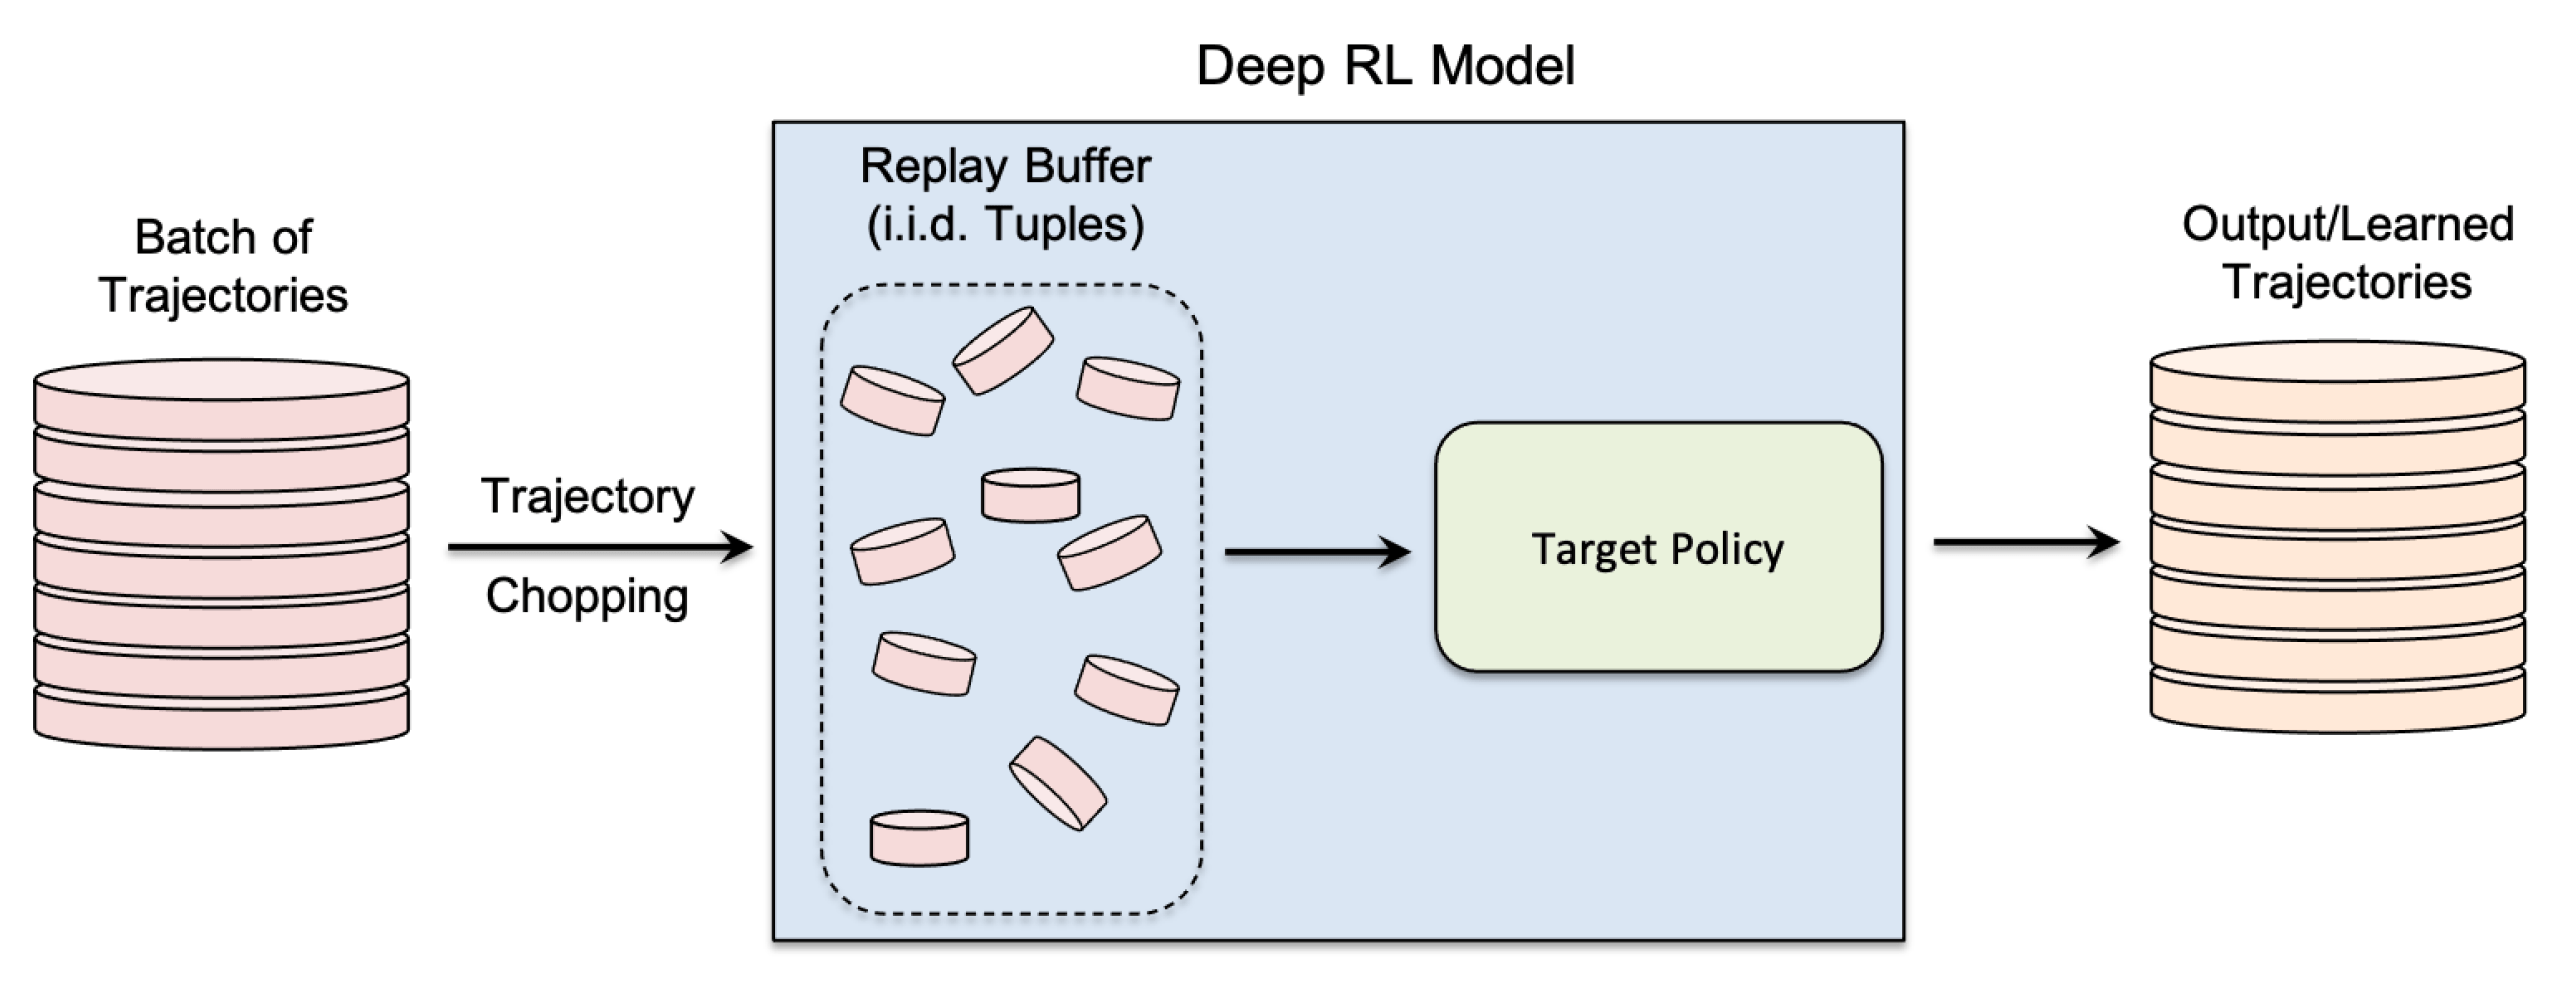
\includegraphics[width=\textwidth]{img/ReplayBuffer.png}
  \end{columns}

  \textbf{Why replay buffer?}
  \begin{itemize}
    \item Breaks temporal correlations in data (notice i.i.d assumption)
    \item Reuse of past experience
    \item Improves sample efficiency
  \end{itemize}

  \vspace{0.8em}

  RL $\rightarrow$ supervised learning by creating targets from experience.
\end{frame}

\begin{frame}{Exploration Strategies}
  \begin{columns}[T]
    \column{0.48\textwidth}
      \textbf{Greedy Policy}\\
      Always pick $a=\arg\max_{a'}Q(s,a')$.\\
      $\Rightarrow$ No exploration; gets stuck.

      \vspace{0.8em}
      \textbf{$\varepsilon$-Greedy}
      \[a = \begin{cases}\text{random} & \text{with prob.\ }\varepsilon\\\arg\max_a Q(s,a) & \text{otherwise}\end{cases}\]
      $\varepsilon$ is annealed over training (explore $\to$ exploit).\\

    \column{0.48\textwidth}
      \textbf{Boltzmann (Softmax) Exploration}
      \[\pi(a|s) = \frac{\exp(Q(s,a)/\tau)}{\sum_{a'}\exp(Q(s,a')/\tau)}\]
      Temperature $\tau$ is annealed over training.\\[0.4em]
      Actions with higher Q-values are \emph{proportionally} more likely — softer than $\varepsilon$-greedy.

  \end{columns}
\end{frame}

\begin{frame}{Target Network: Solving Moving Target Problem}
  \begin{columns}[T]
    \column{0.52\textwidth}
      \textbf{Problem:} Using the \emph{same} network for both prediction and target:
      \[\text{Target} = r + \gamma\max_{a'}Q(s',a';\theta)\]
      Every update shifts the target $\Rightarrow$ feedback loop $\Rightarrow$ oscillation / divergence.

      \vspace{0.6em}
      \textbf{Solution — Target Network $\theta^-$:}
      \begin{itemize}
        \item Identical copy of online network, weights \emph{frozen}
        \item Used \emph{exclusively} to compute TD target
        \item Synced to $\theta$ every $C$ steps: $\theta^- \leftarrow \theta$
      \end{itemize}

    \column{0.45\textwidth}
      \begin{block}{DQN Target}
        \[y^{\text{DQN}} = r + \gamma\max_{a'}Q(s',a';\theta^-)\]
      \end{block}
      \vspace{0.4em}
      \begin{alertblock}{Effect}
        RL temporarily becomes a \emph{supervised} task with a stable objective — decouples weight updates from target calculation.
      \end{alertblock}
  \end{columns}
\end{frame}

\begin{frame}{Double DQN Learner}
  \emph{online} network $Q_\theta$ + \emph{target} network $Q_{\theta^-}$.

  \vspace{0.5em}
  \textbf{Double DQN target} (decouples selection from evaluation):
  \[y_t = r_t + \gamma\, Q_{\theta^-}\!\left(s_{t+1},\;\underbrace{\arg\max_{a'} Q_\theta(s_{t+1},a')}_{\text{online selects action}}\right)(1-d_t)\]

  \vspace{0.5em}
  \begin{columns}[T]
    \column{0.48\textwidth}
      \begin{itemize}
        \item Target sync every \texttt{target\_sync\_interval} epochs
        \item Hard copy ($\tau=1$) by default; optional Polyak averaging
      \end{itemize}
    \column{0.48\textwidth}
      \begin{alertblock}{Why Double DQN?}
        Standard DQN tends to \emph{overestimate} Q-values because the max-operator uses the same network for selection and evaluation. DDQN reduces this bias.
      \end{alertblock}
  \end{columns}
\end{frame}

% ==========================================================
\section{Implementation}
% ==========================================================

\begin{frame}{System Architecture}
  \begin{columns}[c]
    \column{0.6\textwidth}
    \centering
    \includesvg[width=0.75\textwidth]{img/dqn-system-architecture.svg}

    \column{0.4\textwidth}
    \textbf{Key Facts}
    \begin{itemize}
      \item Action Space Discretization (2 bins)
      \item MLP 
      \item Experience Replay Buffer
      \item Target Network Update
      \item greedy, $\epsilon$-greedy \& Boltzmann
      \item Double-DQN
    \end{itemize}
  \end{columns}
\end{frame}

\begin{frame}{Neural Network Architecture}
  \textbf{Multilayer Perceptron (MLP)} approximating $Q^*(s,a)$:

  \vspace{0.6em}
  \begin{center}
    \begin{tabular}{lll}
      \toprule
      \textbf{Key} & \textbf{Hidden layers} & \textbf{Use} \\
      \midrule
      \texttt{mlp\_small}  & $128 \to 128$                    & Ablation baseline \\
      \texttt{mlp\_medium} & $256 \to 128 \to 64$             & Ablation \\
      \texttt{mlp\_large}  & $512 \to 256 \to 128 \to 64$     & Best results \\
      \bottomrule
    \end{tabular}
  \end{center}

  \vspace{0.6em}
  \begin{itemize}
    \item \textbf{Input:} 24-dimensional observation vector
    \item \textbf{Activation:} ReLU after each hidden layer
    \item \textbf{Output:} Q-value per discrete action (one neuron per action index)
    \item Registered in \texttt{NetworkFactory} for easy config-driven selection
  \end{itemize}
\end{frame}

\begin{frame}{Training Loop}
  Each epoch runs 3 phases:

  \vspace{0.5em}
  \begin{enumerate}
    \item \textbf{Collection} — current policy interacts with environment(s) for \texttt{steps\_per\_epoch} steps; transitions stored in buffer.
    \vspace{0.3em}
    \item \textbf{Optimization} — \texttt{updates\_per\_epoch} mini-batches of size \texttt{batch\_size} sampled $\rightarrow$ gradient steps.
    \vspace{0.3em}
    \item \textbf{Target sync} — target network updated every \texttt{target\_sync\_interval} epochs.
  \end{enumerate}
  \vspace{1.0em}
  \textbf{Warmup} — Additionally, the first epoch is preceded by Warmup: Fill replay buffer with randomly sampled experiences, without updating gradients.

\end{frame}

% ==========================================================
\section{Experiment Setup}
% ==========================================================

\begin{frame}{Experimental Setup \& Evaluation Protocol}
  \begin{columns}[c]
    \column{0.5\textwidth}

      \vspace{0.5em}
      \textbf{Metrics reported:}
      \begin{itemize}
        \item Mean \& std of cumulative return
        \item Median, min, max, best
        \item Mean episode length (survival proxy)
      \end{itemize}

    \column{0.47\textwidth}
      \textbf{Hyperparameters:}
      \begin{itemize}
          \item Network $\in$ mlp-\{large, medium, small\}
          \item Exploration Policy
          \item Learning Rate
          \item Discount Factor ($\gamma$)
          \item Replay Buffer Size
          \item Batch Size
          \item Warmup Steps
          \item Target Sync Interval
          \item Exploration ($\epsilon$)
          \item ...
      \end{itemize}
  \end{columns}
\end{frame}

\begin{frame}{Ablation Study Overview}
  Multiple configurations were trained varying one or more hyperparameters at a time:

  \vspace{0.6em}
  \begin{center}
    \begin{tabular}{clp{5.5cm}}
      \toprule
      \textbf{Cat.} & \textbf{Variable} & \textbf{What we tested} \\
      \midrule
      01 & Exploration rate & Baseline vs.\ higher $\varepsilon_{\text{end}}$ ($0.05 \to 0.10$) \\
      02 & Learning rate    & $3{\times}10^{-4}$ vs.\ $10^{-4}$ \\
      03 & Architecture     & \texttt{mlp\_medium} vs.\ \texttt{mlp\_large} \\
      04 & Replay + Batch   & Larger buffer \& batch size combo \\
      05 & Discount $\gamma$ & $0.99$ vs.\ $0.97$ \\
      06 & Exploration type & Boltzmann vs.\ $\varepsilon$-greedy \\
      \bottomrule
    \end{tabular}
  \end{center}
\end{frame}

% ==========================================================
\section{Results and Discussion}
% ==========================================================

\begin{frame}{BipedalWalker: Top 5 runs}
  \begin{center}
    \footnotesize
    \setlength{\tabcolsep}{3pt}
    \begin{tabular}{rlllcllrrrr}
      \toprule
      \textbf{R} & \textbf{Buffer} & \textbf{Start} & \textbf{End} & \textbf{LR} & \textbf{Policy} & \textbf{Mean} & \textbf{Std} & \textbf{Med.} & \textbf{Best} \\
      \midrule
      \textbf{1} & 500k & 2.0 & 0.2 & $5\cdot10^{-5}$ & Boltzmann & \textbf{329.16} & 49.99 & 321.32 & 513.25 \\
      \textbf{2} & 500k & 1.0 & 0.1 & $5\cdot10^{-5}$ & $\varepsilon$-greedy & 243.00 & 50.80 & 229.60 & 413.00 \\
      3 & 200k & 1.0 & 0.1 & $2.5\cdot10^{-4}$ & $\varepsilon$-greedy & 167.95 & 9.42  & 167.20 & 188.44 \\
      4 & 100k & 1.0 & 0.1 & $3\cdot10^{-4}$ & $\varepsilon$-greedy & 163.71 & 12.57 & 164.61 & 189.30 \\
      5 & 200k & 2.5 & 0.1 & $2.5\cdot10^{-4}$ & Boltzmann & 160.57 & 14.96 & 159.09 & 195.71 \\
      \bottomrule
    \end{tabular}
  \end{center}
  \vspace{0.5em}
  \small
  
  \vspace{0.2em}
  At similar settings there are no big differences between runs.
\end{frame}

\begin{frame}{Findings}
  \begin{columns}[T]
    \column{0.5\textwidth}

    \begin{itemize}

      \item \textbf{Boltzmann Exploration:} Best results, but required extensive tuning.
      \begin{itemize}
        \item Proportional exploration: better actions explored more often
        \item Avoids purely random, wasteful moves
        \item Richer learning signal
      \end{itemize}
      \item $\epsilon$-Greedy achieved the lowest standard deviation.
      \begin{itemize}
        \item Stable and predictable
        \item Lower performance ceiling
      \end{itemize}
    \end{itemize}

    \column{0.5\textwidth}
    \begin{itemize}

      \item \textbf{MLP capacity} most important factor
      \begin{itemize}
        \item \texttt{mlp\_large} $\gg$ \texttt{mlp\_medium}
      \end{itemize}
      \item Discount factor $\gamma$ strongly influences long-term planning.
      \item Learning rate is highly sensitive and requires tuning.
      \item Long-horizon discount ($\gamma=0.99$) is beneficial.
      \item Large network and large replay buffer good

    \end{itemize}

  \end{columns}
\end{frame}

\begin{frame}{Successful Parameters}

\textbf{Observation:} Long plateau and abrupt rise.

\vspace{0.8em}

\begin{columns}[c]

  \column{0.33\linewidth}
  \centering
  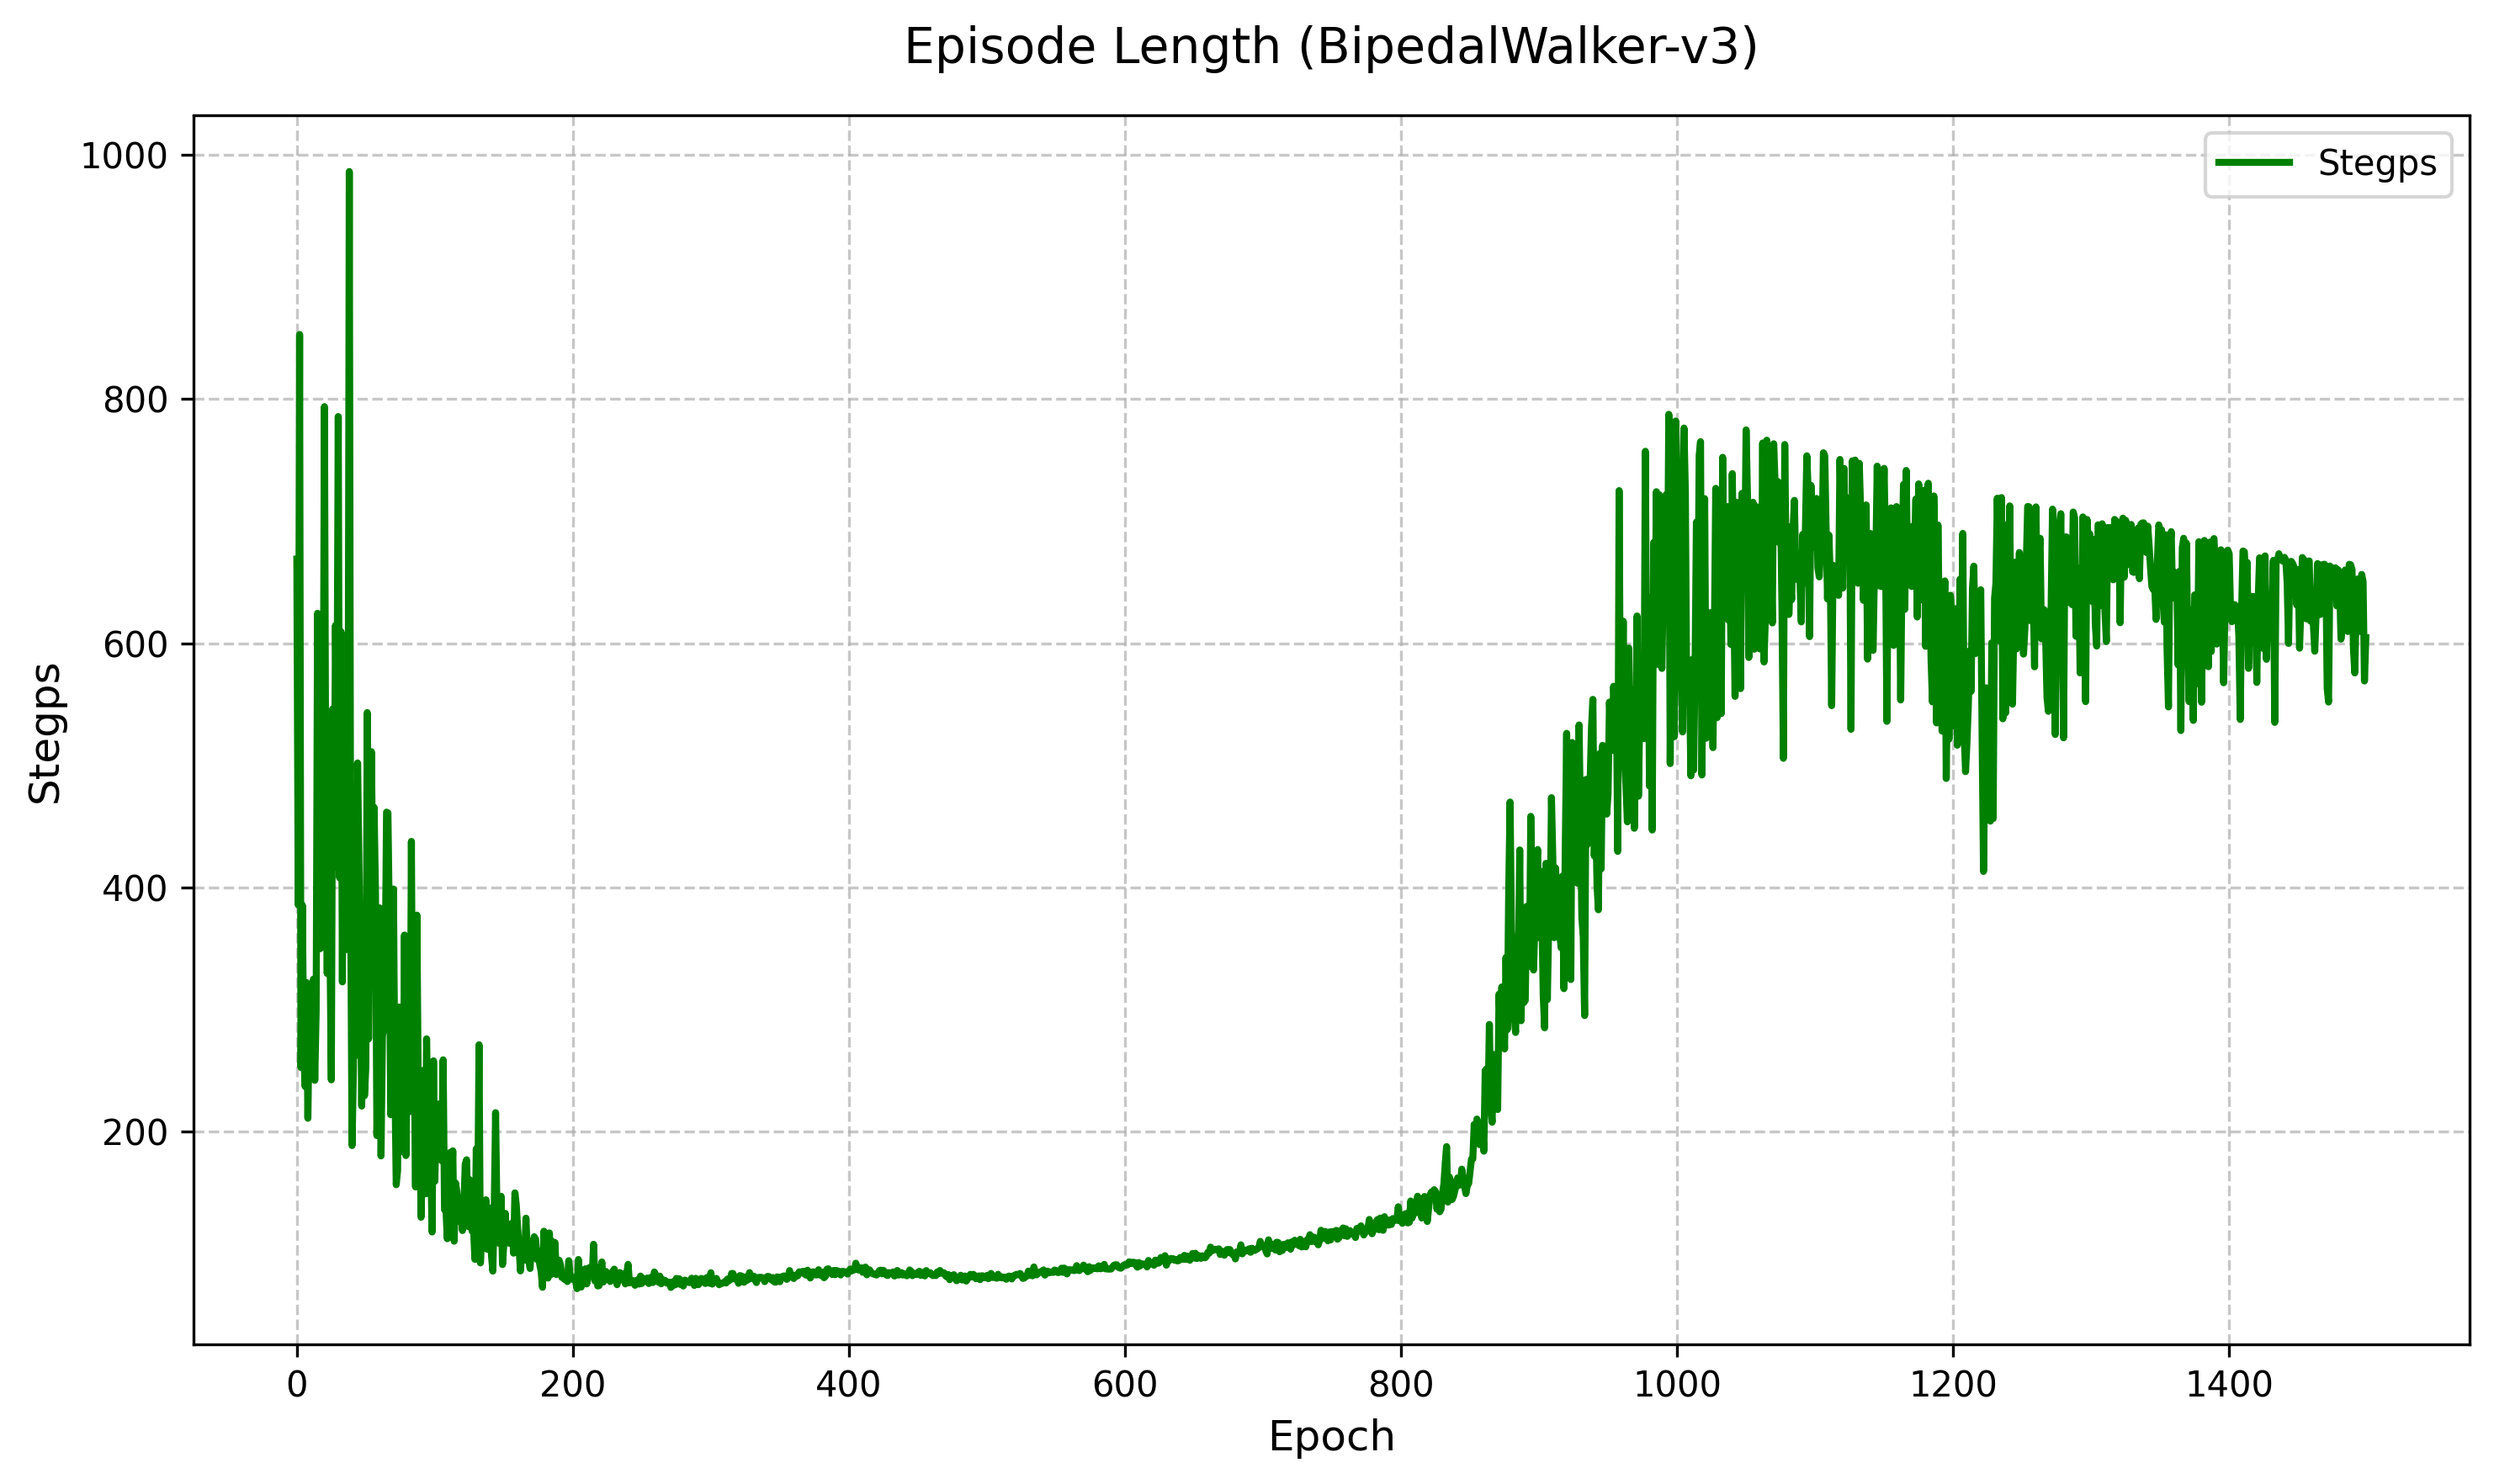
\includegraphics[width=0.7\linewidth]{img/bw-success-length.png}
  \tiny Ep. Length

  \column{0.33\linewidth}
  \centering
  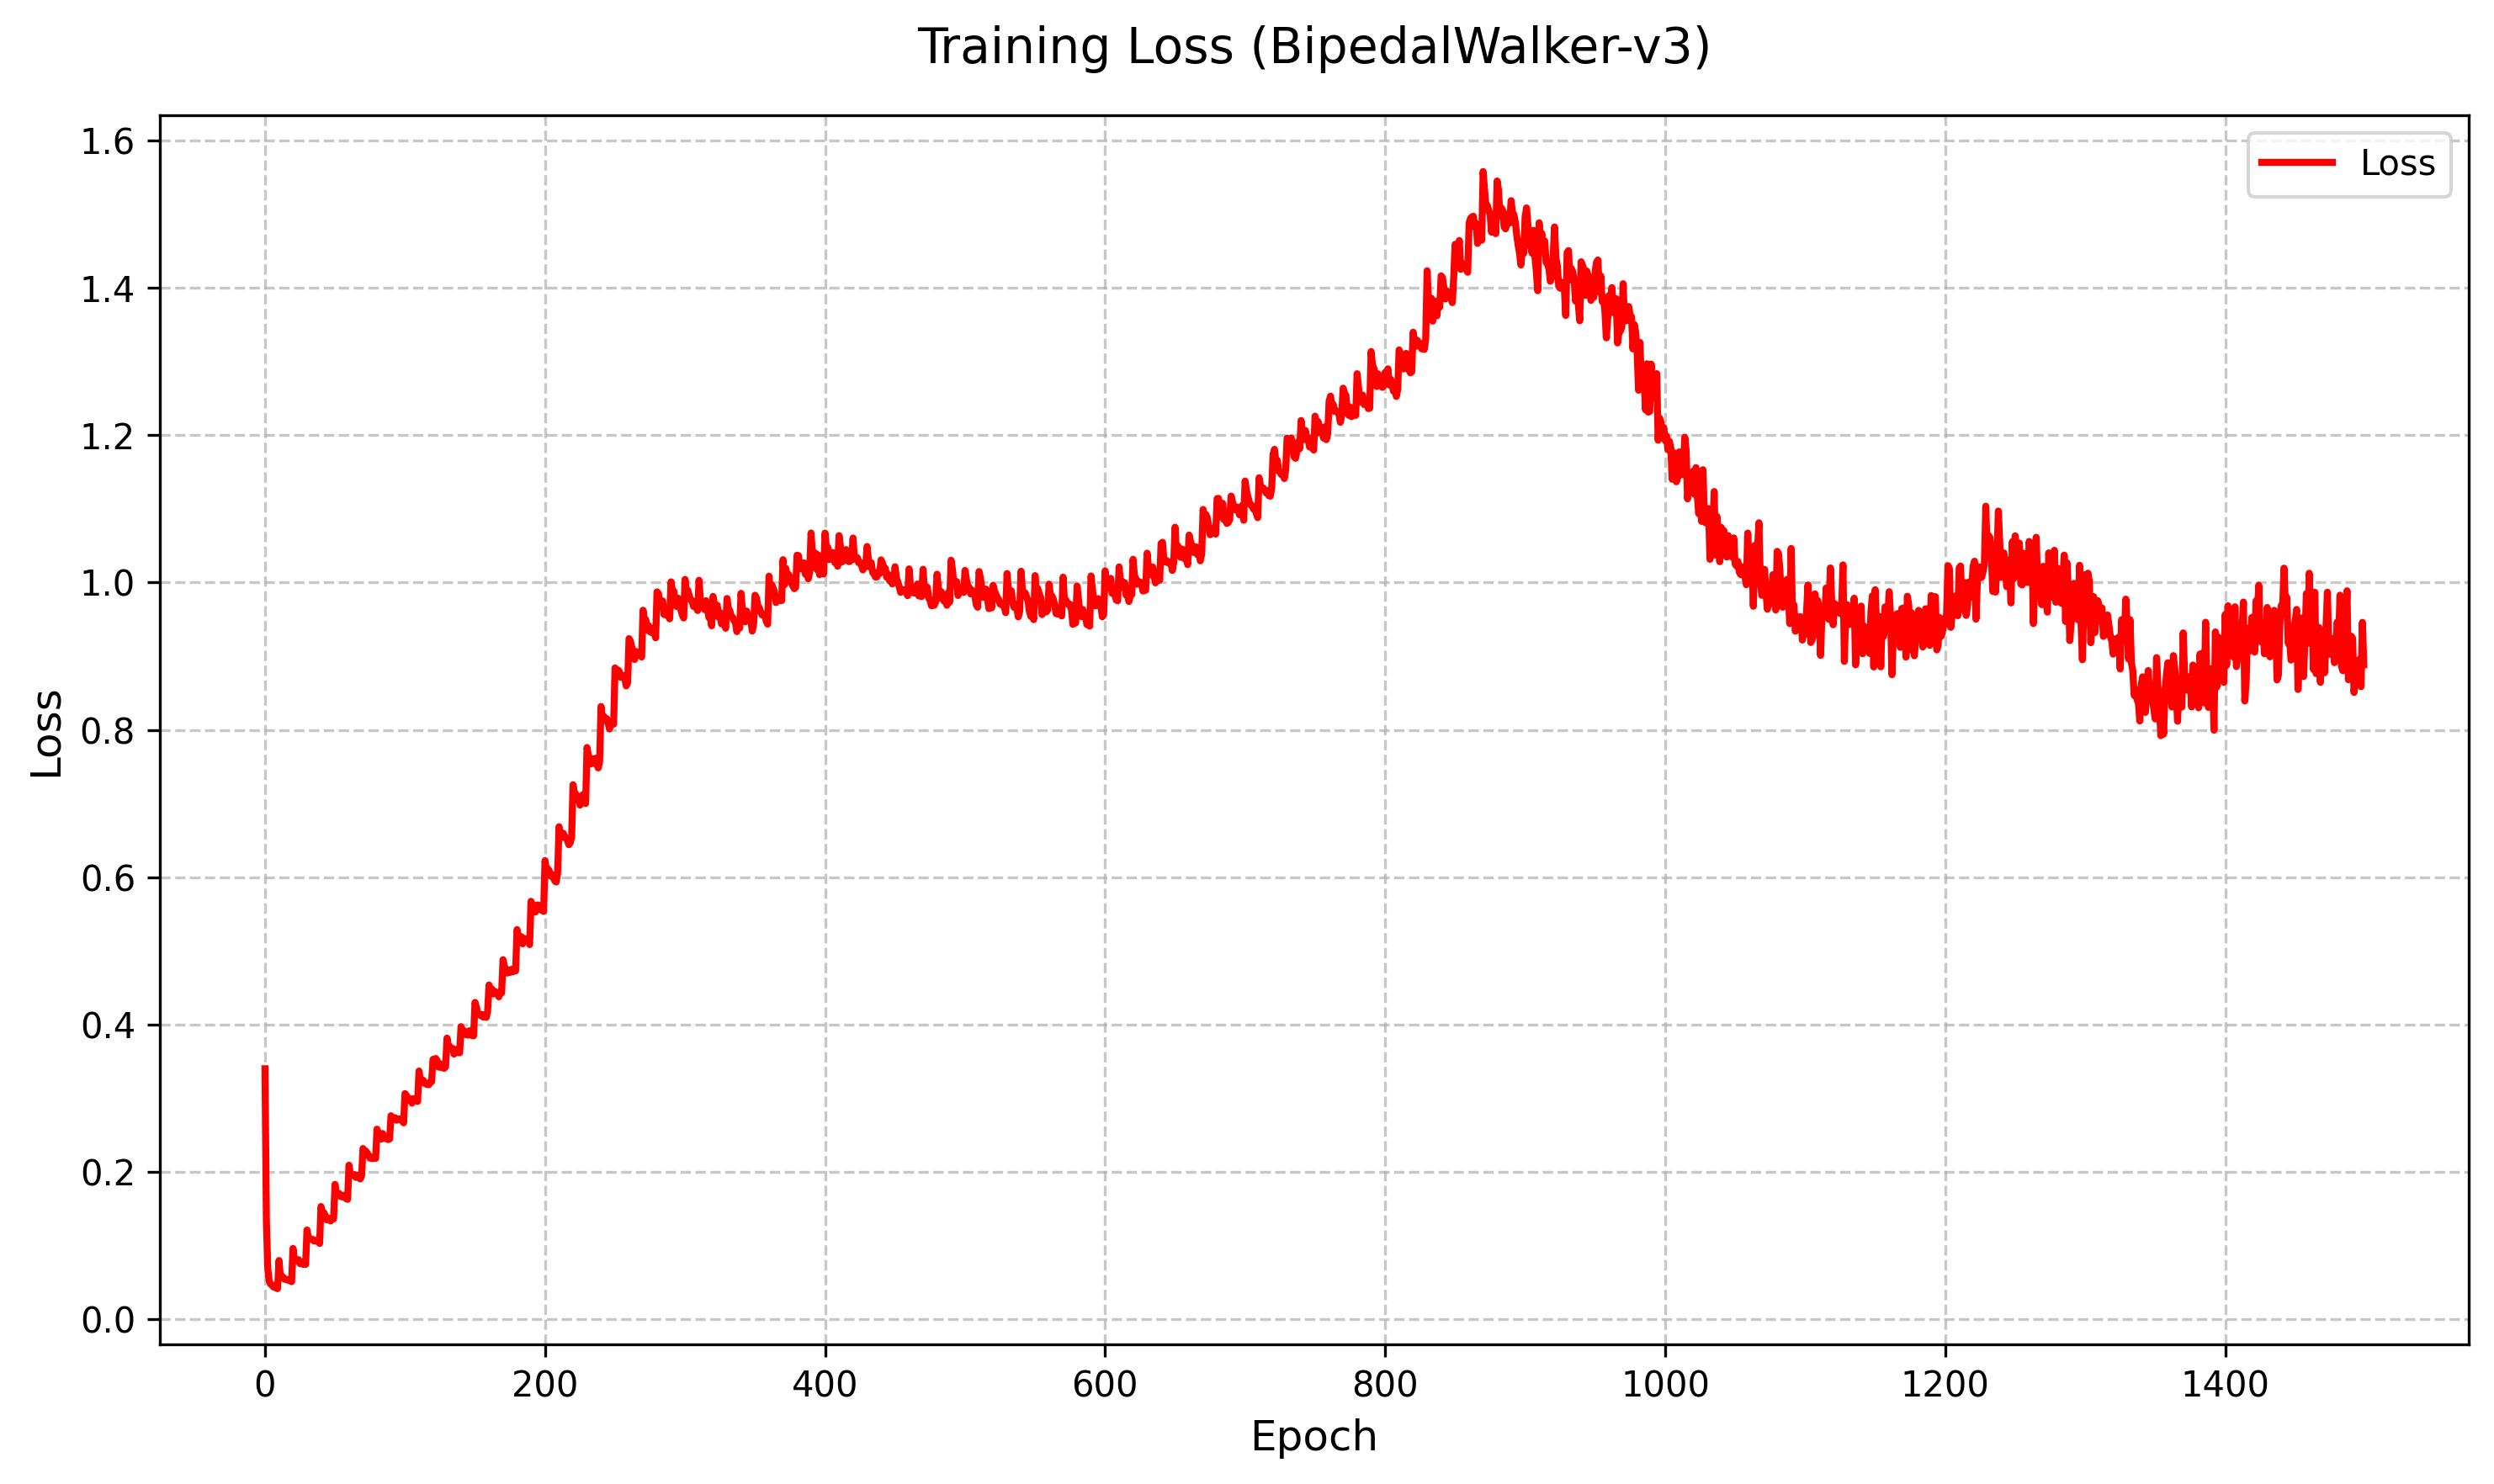
\includegraphics[width=0.7\linewidth]{img/bw-success-loss.png}
  \tiny Ep. Loss

  \column{0.33\linewidth}
  \centering
  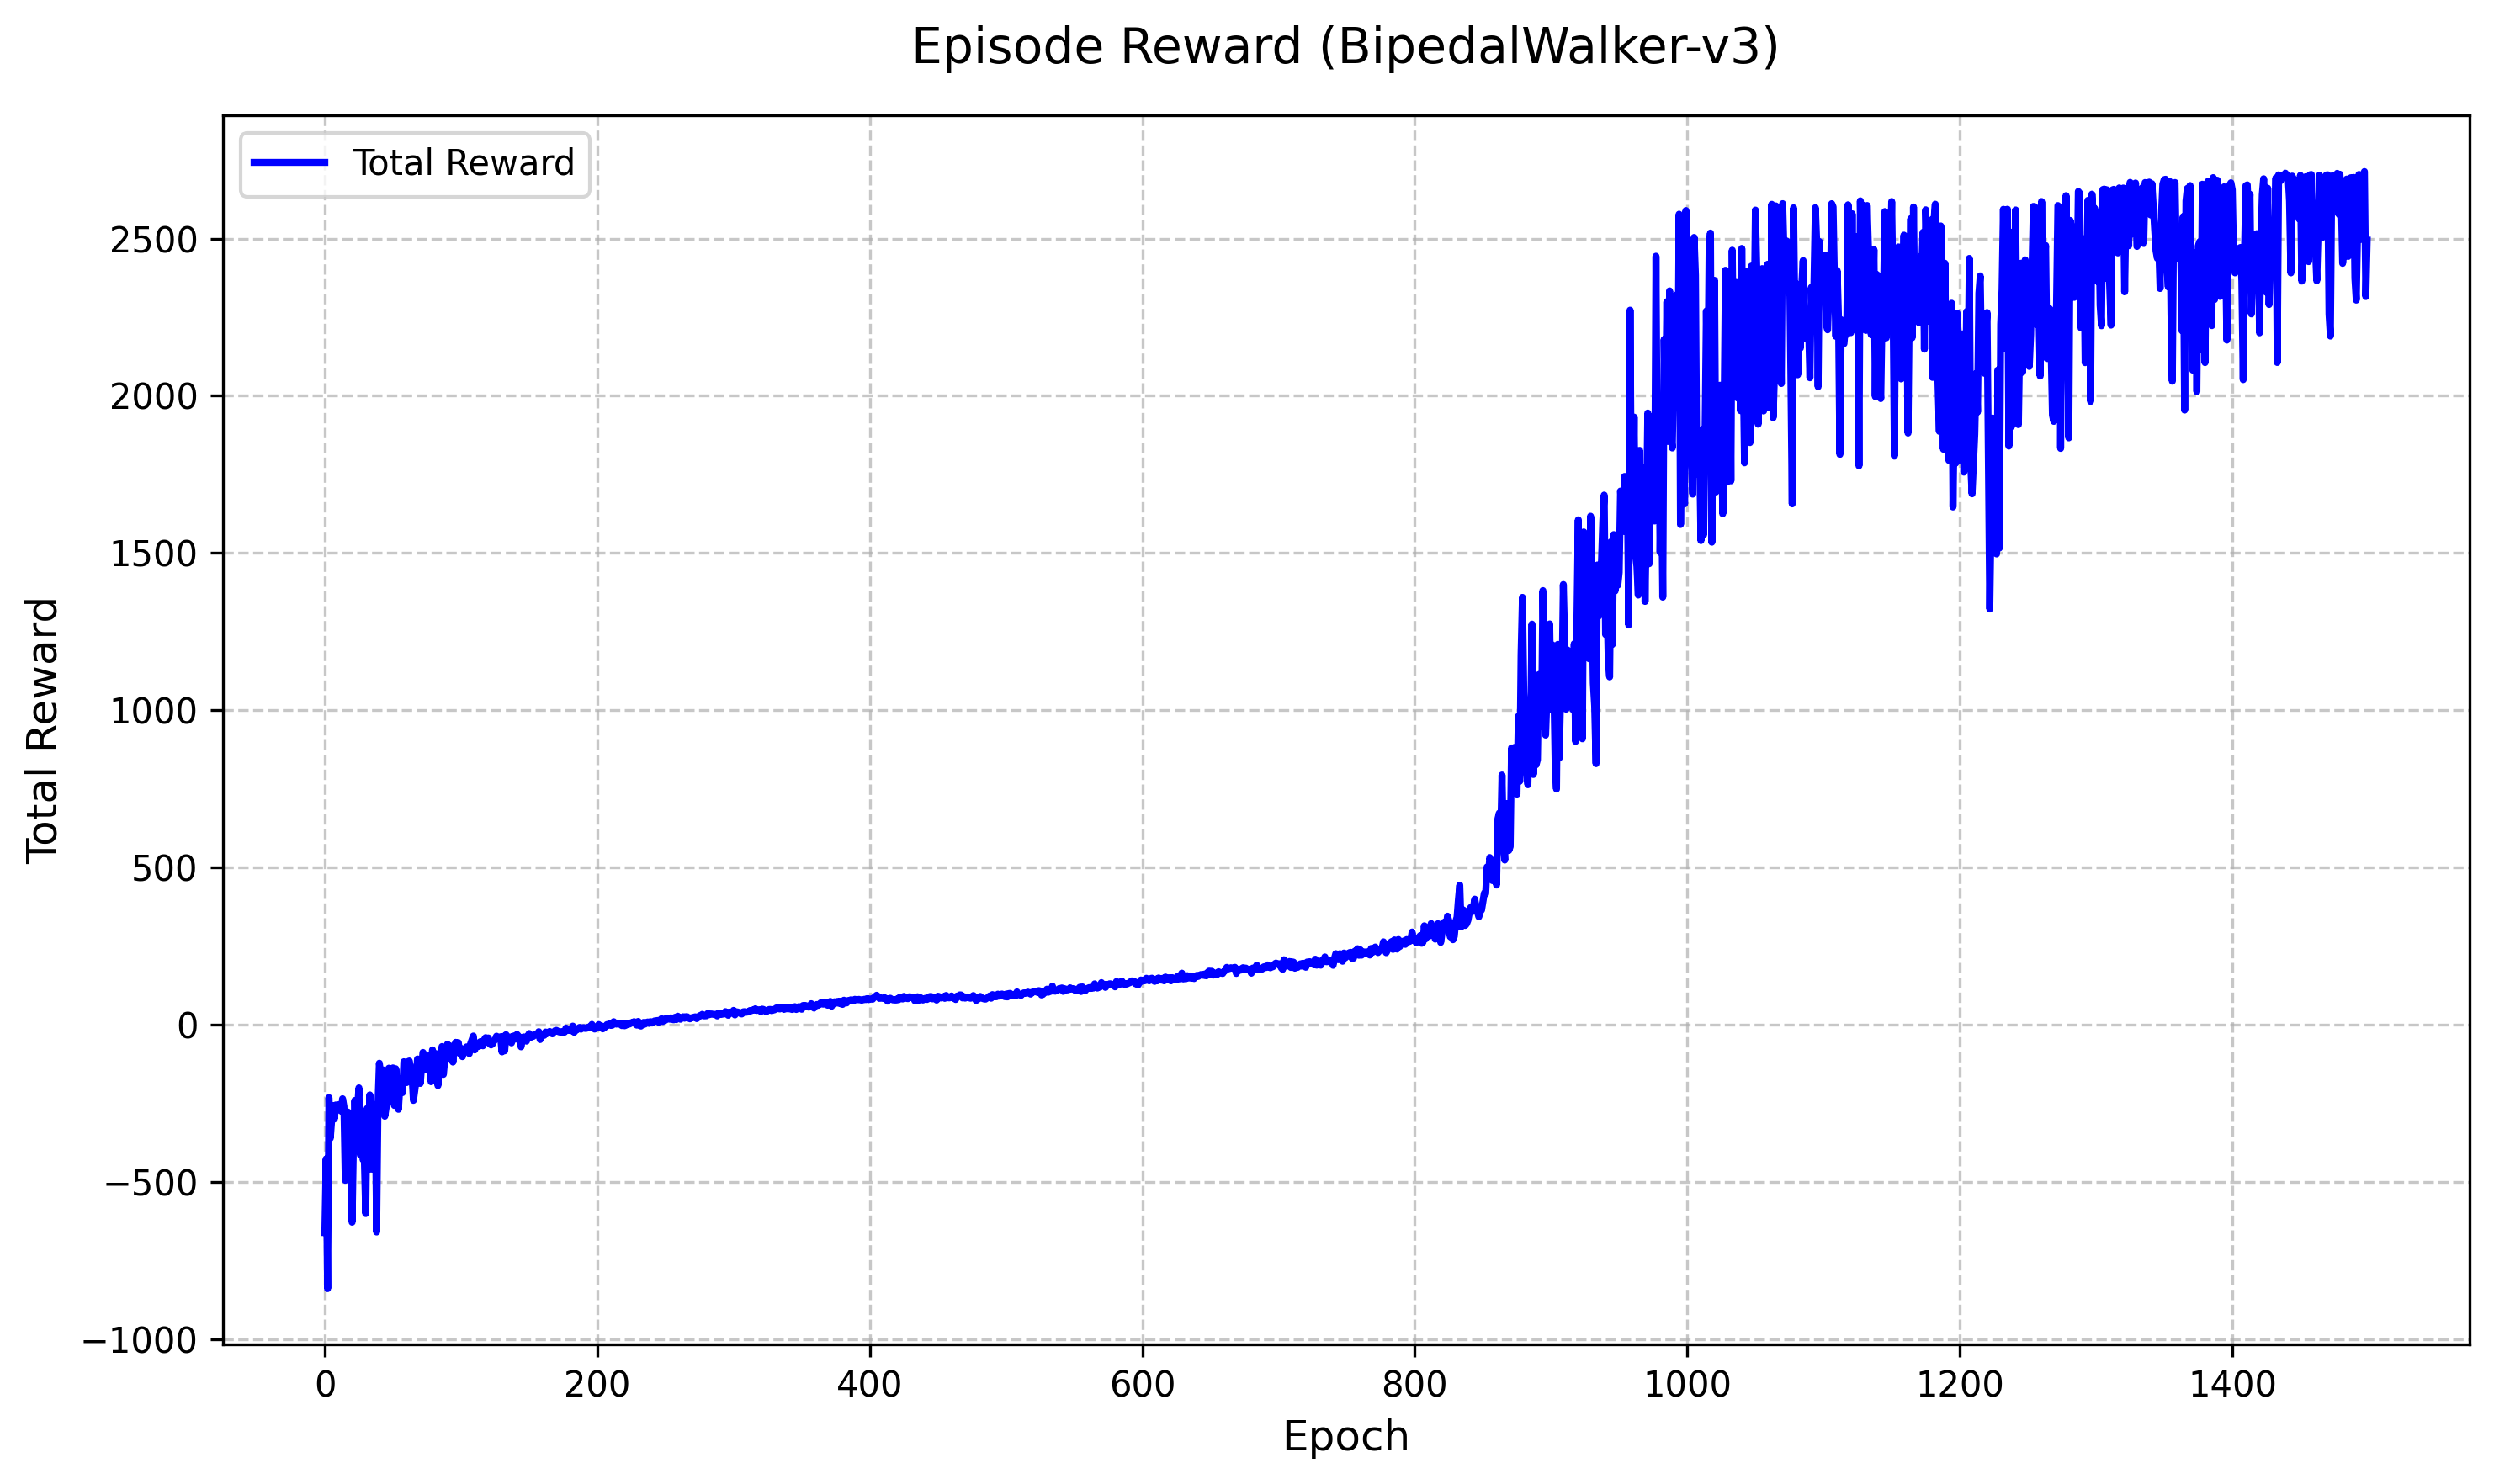
\includegraphics[width=0.7\linewidth]{img/bw-success-reward.png}
  \tiny Ep. Reward

\end{columns}

\vspace{1.0em}

\begin{columns}[T]
  \column{0.4\linewidth}

  \textbf{Key dynamics:}
  \begin{itemize}
    \item \footnotesize Loss increases initially, then decreases as reward shoots up.
    \item \footnotesize Episode length increases alongside reward
  \end{itemize}

  \textbf{Best Model:}
  \begin{itemize}
    \item \footnotesize Solved Episode Length: $329.16 \geq 300$
    \item \footnotesize mlp\_large + Boltzman
  \end{itemize}

  \column{0.5\linewidth}
  \renewcommand{\arraystretch}{1.2}
  \scriptsize
  \begin{tabular}{ll}
  \textbf{Component} & \textbf{Value} \\
    \hline
    Network / Policy & mlp\_large + Boltzmann \\
    Learning rate & $5 \times 10^{-5}$ \\
    Discount factor ($\gamma$) & 0.99 \\
    Batch size & 256 \\
    Replay buffer & 500k \\
    Warmup & 50k steps \\
    Training setup & 1500 epochs, 1000 stp./ep. \\
    Exploration & 2.0 $\rightarrow$ 0.2 \\
    Target sync & every 10 updates \\
  \end{tabular}
\end{columns}

\end{frame}

\begin{frame}{Comparative: BipedalWalker vs. BipedalWalkerHardcore}
  How suitable is DQN for   \textbf{Hardcore Variant}? \\
  \vspace{0.75em}
  \begin{columns}[c]
    \column{0.4\linewidth}
    \begin{itemize}
      \item \footnotesize Very uneven terrain.
      \item \footnotesize obstacles, stairs, pits
      \item \footnotesize Higher exploration requirements
    \end{itemize}

    \column{0.6\linewidth}
    \begin{itemize}
      \item \footnotesize Obstacles $\rightarrow$ agent must learn more ``when then'' scenarios.
      \item \footnotesize World model would be good.
      \item \footnotesize Continues action space would be good.
    \end{itemize}
     
  \end{columns}
  \vspace{1.0em}
  \centering
  \small

  \begin{columns}[c]
    \column{0.33\linewidth}
    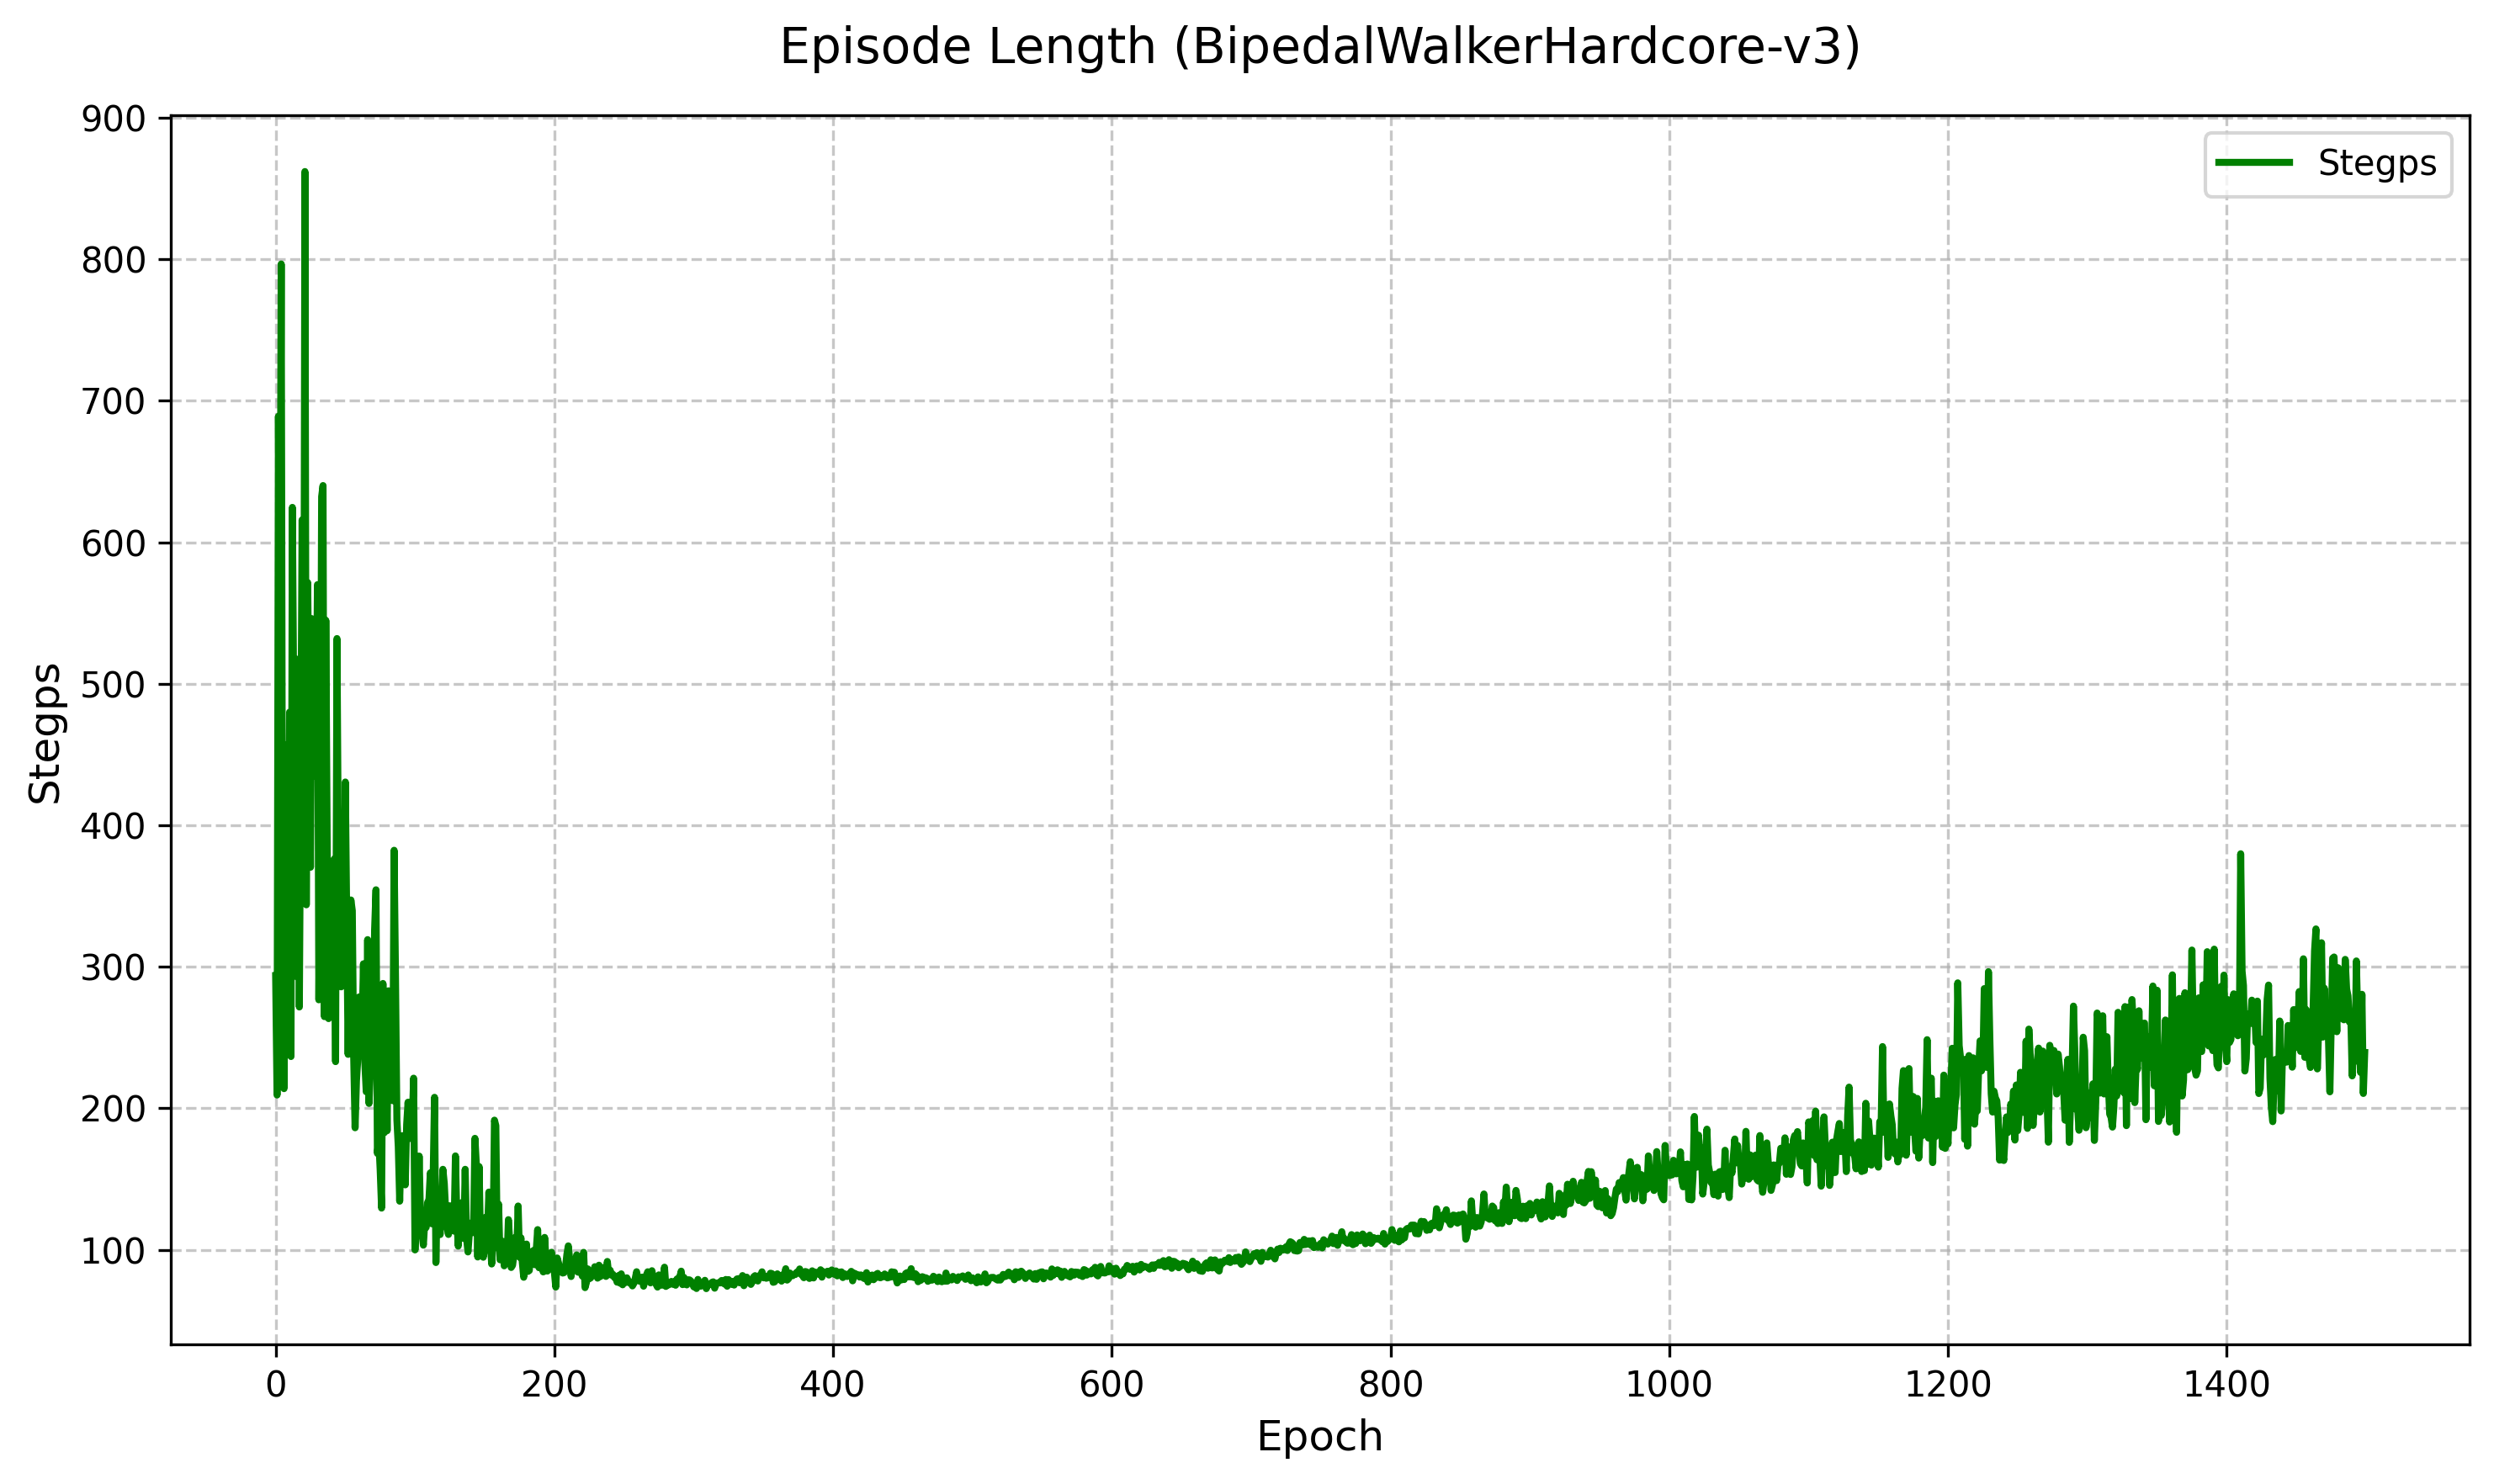
\includegraphics[width=\linewidth]{img/bwh-bw-length.png}
    \column{0.33\linewidth}
    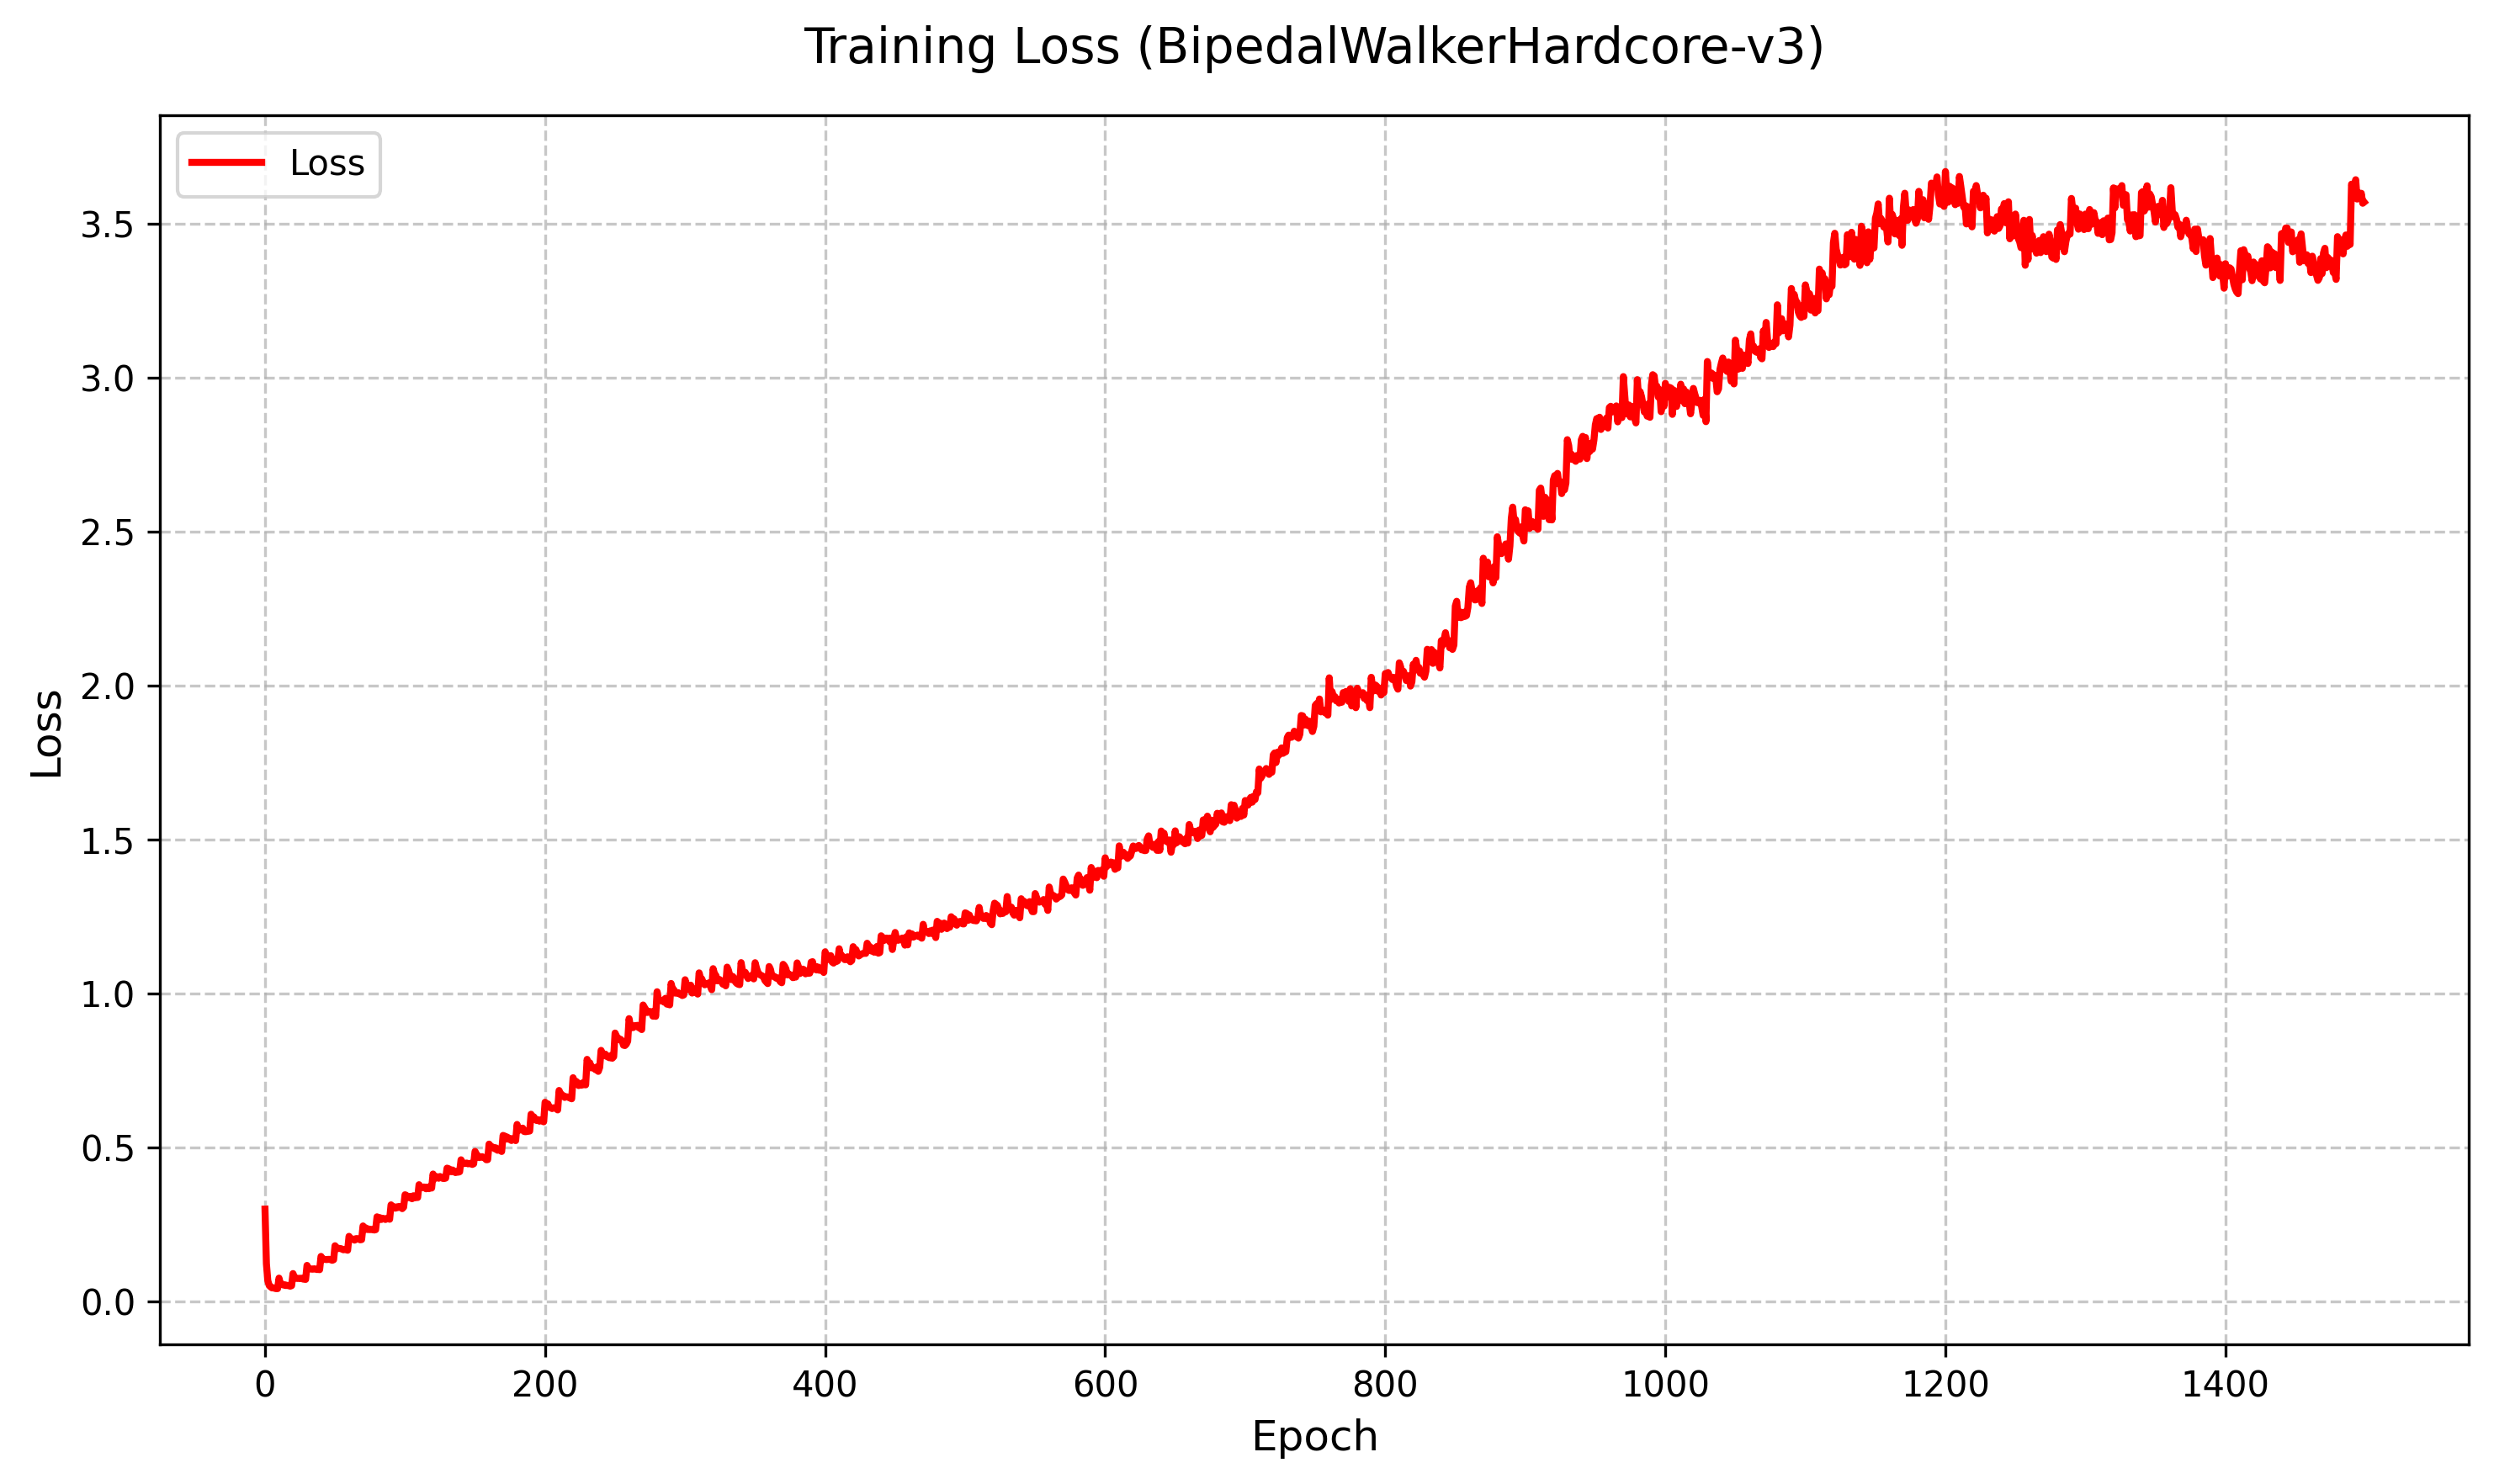
\includegraphics[width=\linewidth]{img/bwh-bw-loss.png}
    \column{0.33\linewidth}
    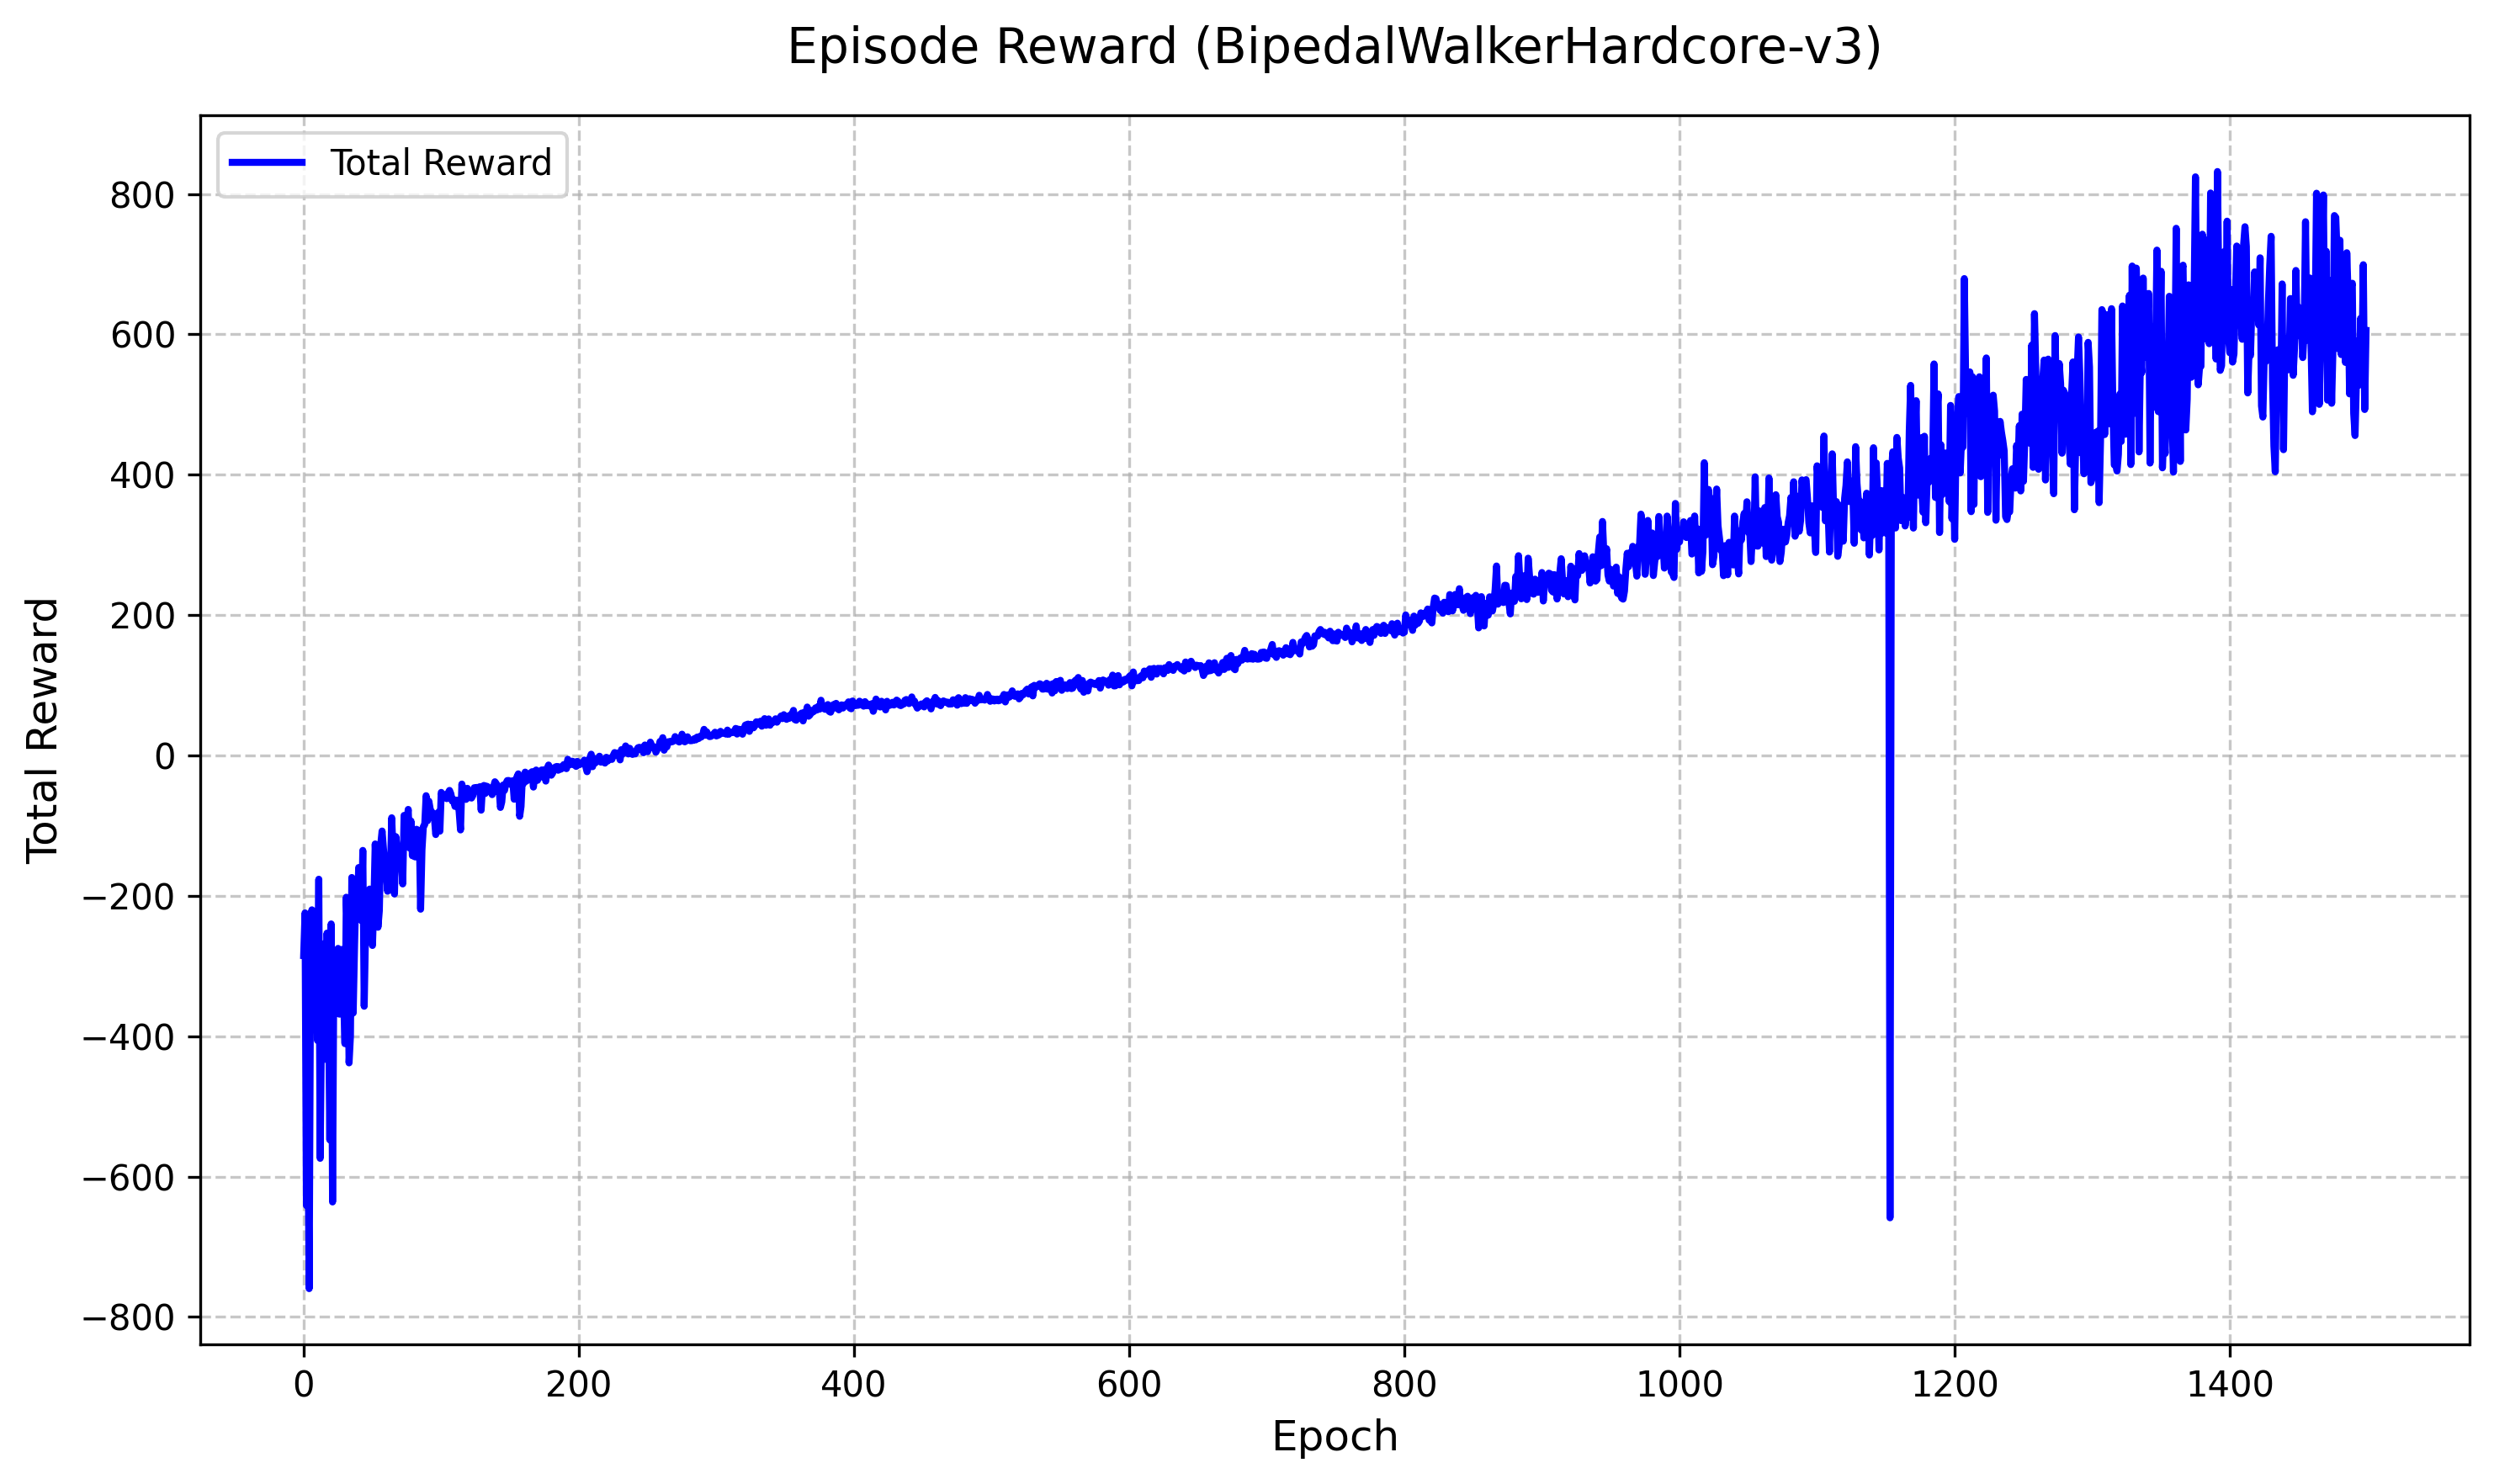
\includegraphics[width=\linewidth]{img/bwh-bw-reward.png}
  \end{columns}
  \vspace{1.5em}
  \begin{center}
    Same params as in ``Default'' variant (see above), do not bring episode length up well, agent fails $\rightarrow$ better hyperparams necessary.
  \end{center}
\end{frame}



\begin{frame}{Bonus: Successful CartPole Parameters}

For comparative we also tested a different environment, CartPole-v1. 

\vspace{0.8em}

\begin{columns}[c]

  \column{0.33\linewidth}
  \centering
  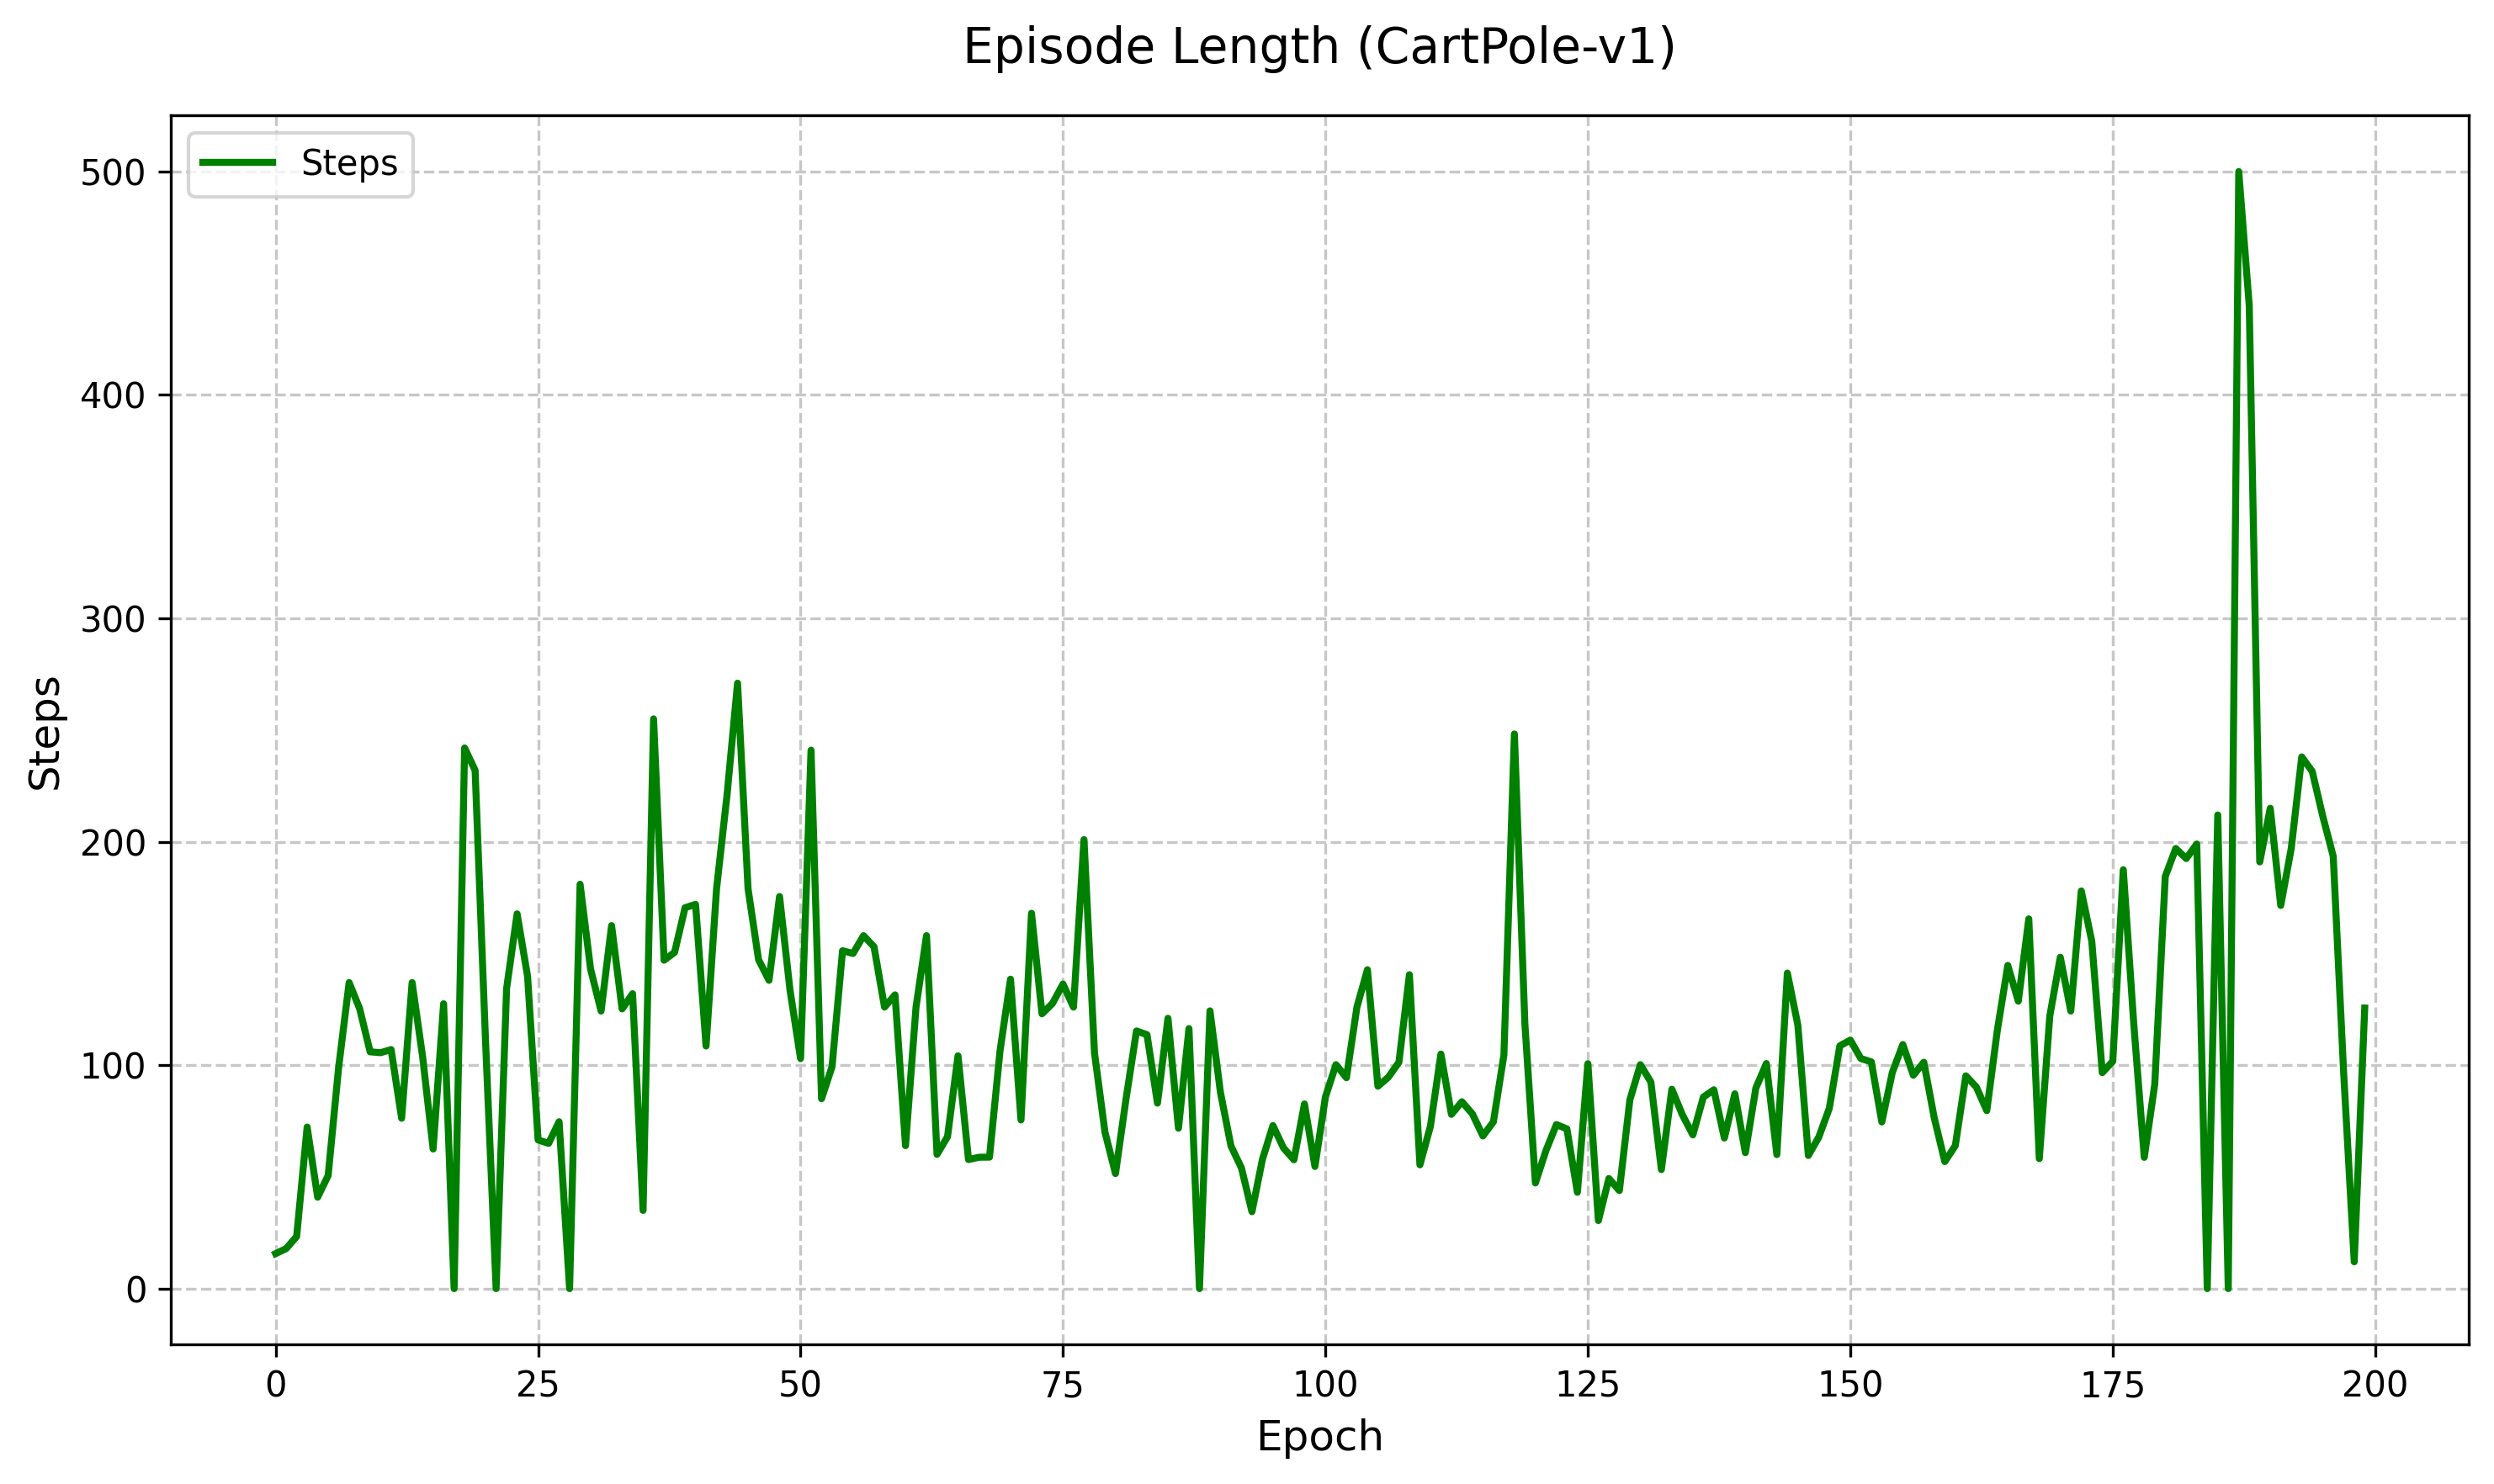
\includegraphics[width=0.7\linewidth]{img/cp-success-epsilon-length.png}
  \tiny Ep. Length

  \column{0.33\linewidth}
  \centering
  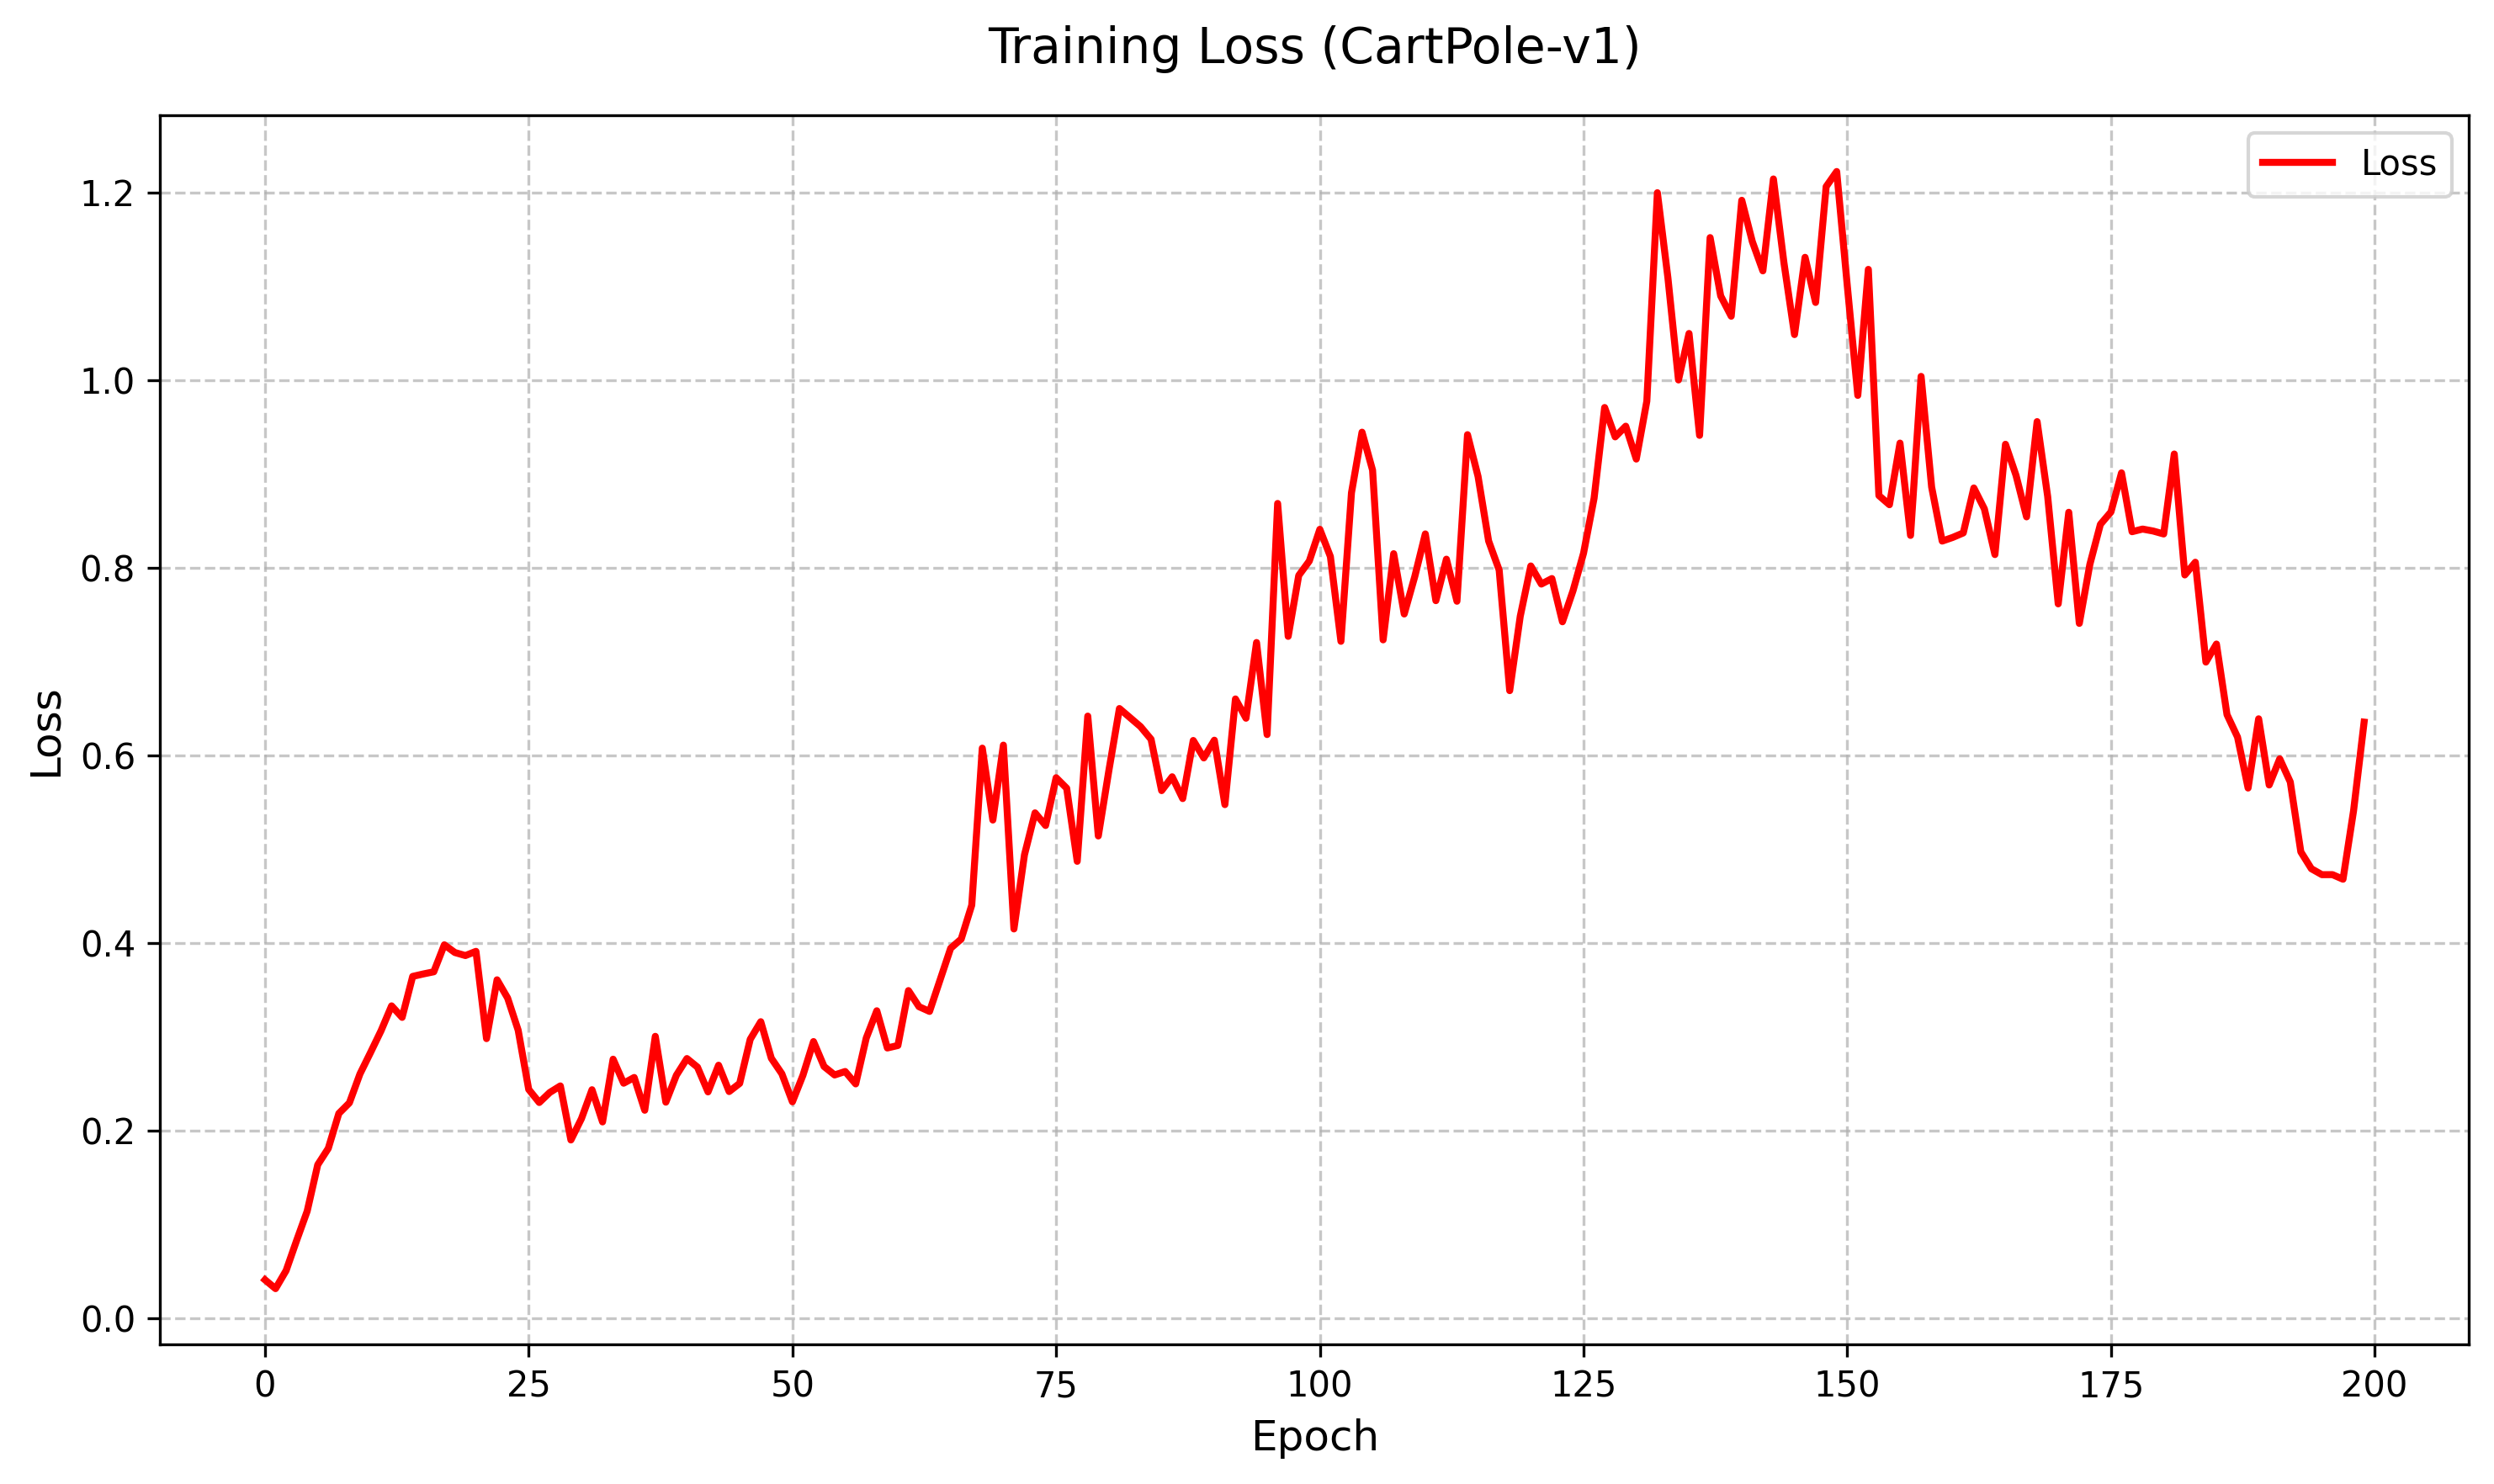
\includegraphics[width=0.7\linewidth]{img/cp-success-epsilon-loss.png}
  \tiny Ep. Loss

  \column{0.33\linewidth}
  \centering
  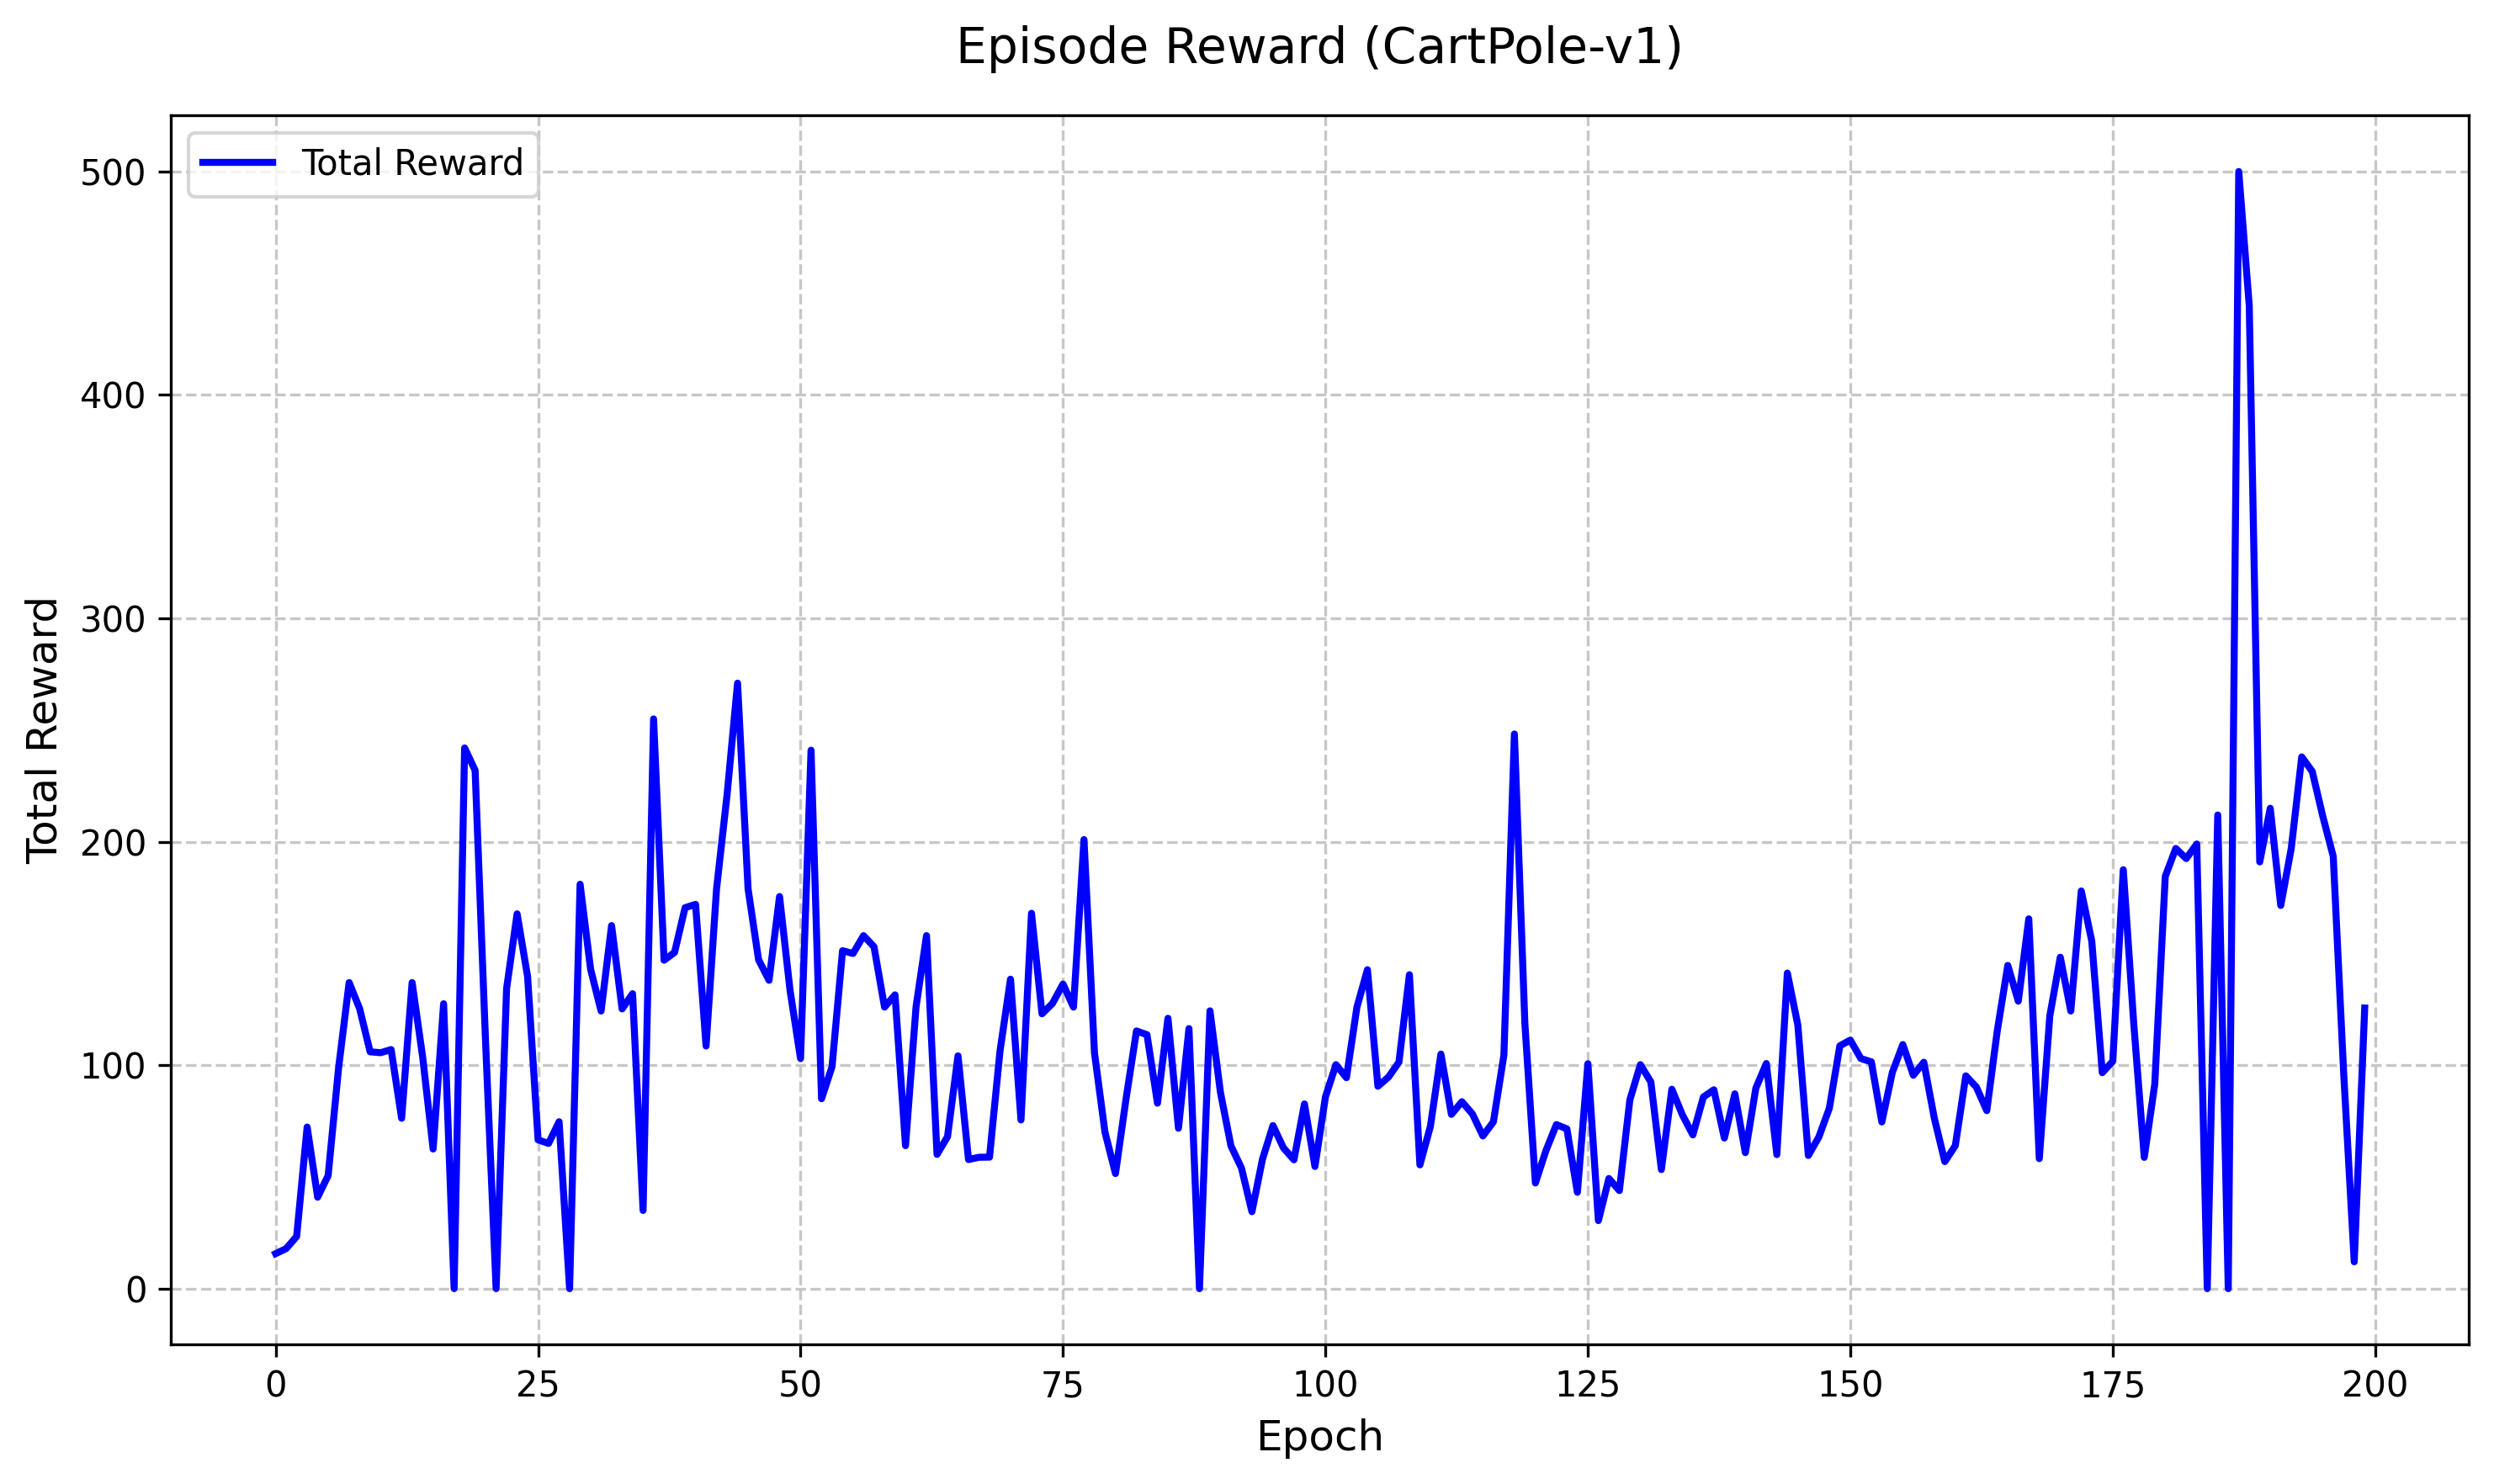
\includegraphics[width=0.7\linewidth]{img/cp-success-epsilon-reward.png}
  \tiny Ep. Reward

\end{columns}

\vspace{1.0em}

\begin{columns}[T]
  \column{0.4\linewidth}

  \textbf{CartPole-v1}
  \begin{itemize}
    \item \footnotesize State: 4D | Action: 2D
    \item \footnotesize Task: Inverse pendelum on cart stabilization
    \item \footnotesize Action Space: already Discrete by default
  \end{itemize}

\textbf{Best Model:}
  \begin{itemize}
    \item \footnotesize Solved Episode Length: $500 \geq 500$ 
    \item \footnotesize mlp\_small + $\epsilon$-greedy
  \end{itemize}


  \vspace{0.5em}

  \column{0.5\linewidth}
  \renewcommand{\arraystretch}{1.2}
  \scriptsize
  \begin{tabular}{ll}
  \textbf{Component} & \textbf{Value} \\
    \hline
    Network / Policy & mlp\_small + $\epsilon$-greedy \\
    Learning rate & $1 \times 10^{-3}$ \\
    Discount factor ($\gamma$) & 0.99 \\
    Batch size & 64 \\
    Replay buffer & 10k \\
    Warmup & 1000 steps \\
    Training setup & 200 epochs, 1k stp/ep., 200 upd./ep. \\
    Exploration & 0.5 $\rightarrow$ 0.05 \\
    Target sync & every update \\
  \end{tabular}
\end{columns}

\end{frame}

\begin{frame}{Comparative: CartPole vs. BipedalWalker}
  \vspace{0.5em}
  Are params for high complexity good in low complexity?
  \vspace{1.0em}
  \begin{columns}[t]
    \column{0.48\textwidth} 
    \textbf{CartPole-v1}
    \begin{itemize}
      \item \footnotesize Simple Stabilization
    \end{itemize}
    \column{0.48\textwidth}
    \textbf{BipedalWalker-v3}
    \begin{itemize}
      \item \footnotesize Task: Complex locomotion
    \end{itemize}
  \end{columns}

  \vspace{1.0em}
  \centering
  \small

  \begin{tabular}{@{}llll@{}}
    \toprule
    {} & \textbf{CartPole} & \textbf{Bipedal} & {} \\ \midrule
    Learning rate & $10^{-3}$ & $5 \cdot 10^{-5}$ & BW Rougher Q-landscape \\
    Exploration & $\epsilon$-greedy & Boltzmann & CP Needs stable Q-values \\
    Network & mlp\_small & mlp\_large & BW must approx. more complex function \\
    Replay Buffer & 10k & 500k & Larger state diversity \\ 
    \bottomrule
  \end{tabular}

  \vspace{1.0em}
  \begin{center}
    \begin{itemize}
      \item \footnotesize Training CartPole with (best) Bipedal params achieves Return of 500 but training unnecessary long \& expensive.
      \item \footnotesize Also Intuitively: $\exists$ simple calssical control with PID $\Rightarrow$ Simple DQN should exist. 
    \end{itemize}
  \end{center}
\end{frame}

\begin{frame}[plain]
    \begin{center}
      \textbf{Roles} \\
      \vspace{0.3em}
      \begin{tabular}{ll}
        Lea Seifried:     Training \\[0.3em]
        Michael Hagmann:  Model \\[0.3em]
        Dominik Rzecki:   Documentation, Slides \\
      \end{tabular}

      \vspace{1.0em}

      \textbf{GenAI usage notice} \\
      \vspace{0.3em}
      \begin{itemize}
        \item drafting of code \& of documentation
        \item explanations \& spec knowledge
      \end{itemize}
    \end{center}
\end{frame}

\begin{frame}{References}
  \begin{center}
    \href{https://www.youtube.com/watch?v=VnpRp7ZglfA}
         {The FASTEST introduction to Reinforcement Learning on the internet}

    \vspace{0.5em}

    Hasselt, Guez, Silver, ``Deep Reinforcement Learning with Double Q-Learning'', Dec.~2015
  \end{center}
\end{frame}

\begin{frame}[plain]
  \begin{center}
    {\Large \textbf{Thank You!}}\\[1.5em]
    \large Questions?\\[2em]
    \normalsize
    \begin{tabular}{ll}
      Lea Seifried:     & \texttt{e12428595@student.tuwien.ac.at} \\[0.3em]
      Michael Hagmann:  & \texttt{e12426877@student.tuwien.ac.at} \\[0.3em]
      Dominik Rzecki:   & \texttt{e12410100@student.tuwien.ac.at} \\
    \end{tabular}
  \end{center}
\end{frame}

\appendix

%\begin{frame}{Appendix: Reward Shaping}
%\small
%\begin{columns}[T]
%
%% Left
%\begin{column}{0.55\textwidth}
%\textbf{Shaped Reward:}
%\begin{equation*}
%r = r_{\text{base}} - 2|\theta| - 0.5|\omega| - 0.5|v_y|
%+ \begin{cases}
%5v_x & v_x > 0 \\
%-0.3 & v_x \le 0
%\end{cases}
%\end{equation*}
%
%\textbf{Motivation:}
%\begin{itemize}\setlength\itemsep{2pt}
%\item Fix sparse reward / local optima (raw $130\Delta x$ fails)
%\item Stabilize posture ($\theta,\omega,v_y$ penalties)
%\item Encourage forward motion, penalize stagnation
%\end{itemize}
%\end{column}
%
%% Right
%\begin{column}{0.45\textwidth}
%\textbf{Gait Constraints:}
%\begin{itemize}\setlength\itemsep{3pt}
%\item \textbf{Foot contact duration}  
%$-0.1(\text{steps}-15)$ per leg
%
%\item \textbf{High contact EMA}  
%$-1.5(\text{EMA}-0.75)$ per leg
%
%\item \textbf{Asymmetry penalty}  
%$-(|\text{EMA}_1-\text{EMA}_2|-0.3)$
%
%\item \textbf{Hip inactivity}  
%$-0.3$ if one hip inactive
%\end{itemize}
%\end{column}
%
%\end{columns}
%\end{frame}

\end{document}
